\chapter{双频激光干涉仪的环境误差补偿实验系统}
%\section{双频激光干涉仪测量系统光路设计与分析}
\section{基于PT100的八通道温度测量系统}
本文工作所采用的温度传感器为基于PT100电阻的多通道温度测量系统,最多支持8个通道的同时测量,供电电压为+12$\sim$+24VDC,能够支持\(22^{\circ} \mathrm{C} \pm 5^{\circ} \mathrm{C}\)范围内的温度测量,测量精度\(\leq \pm 0.04^{\circ} \mathrm{C}\)。

\subsection{上位机系统}
基于PT100电阻的多通道温度测量系统上位机采用美国国家仪器(NI)公司研制的LabVIEW程序开发环境开发,并且需要NI LabVIEW Runtime和NI-VISA模组。该上位机软件能够实现数据的测量、显示、存储并且自带标定数据分析功能,包含一个主vi:main.vi和两个子vi:数据处理.vi和数据存储.vi,上位机软件流程图以及部分关键代码如图\ref{fig:上位机程序示意图}所示。
\begin{figure}[htb]
    \centering
    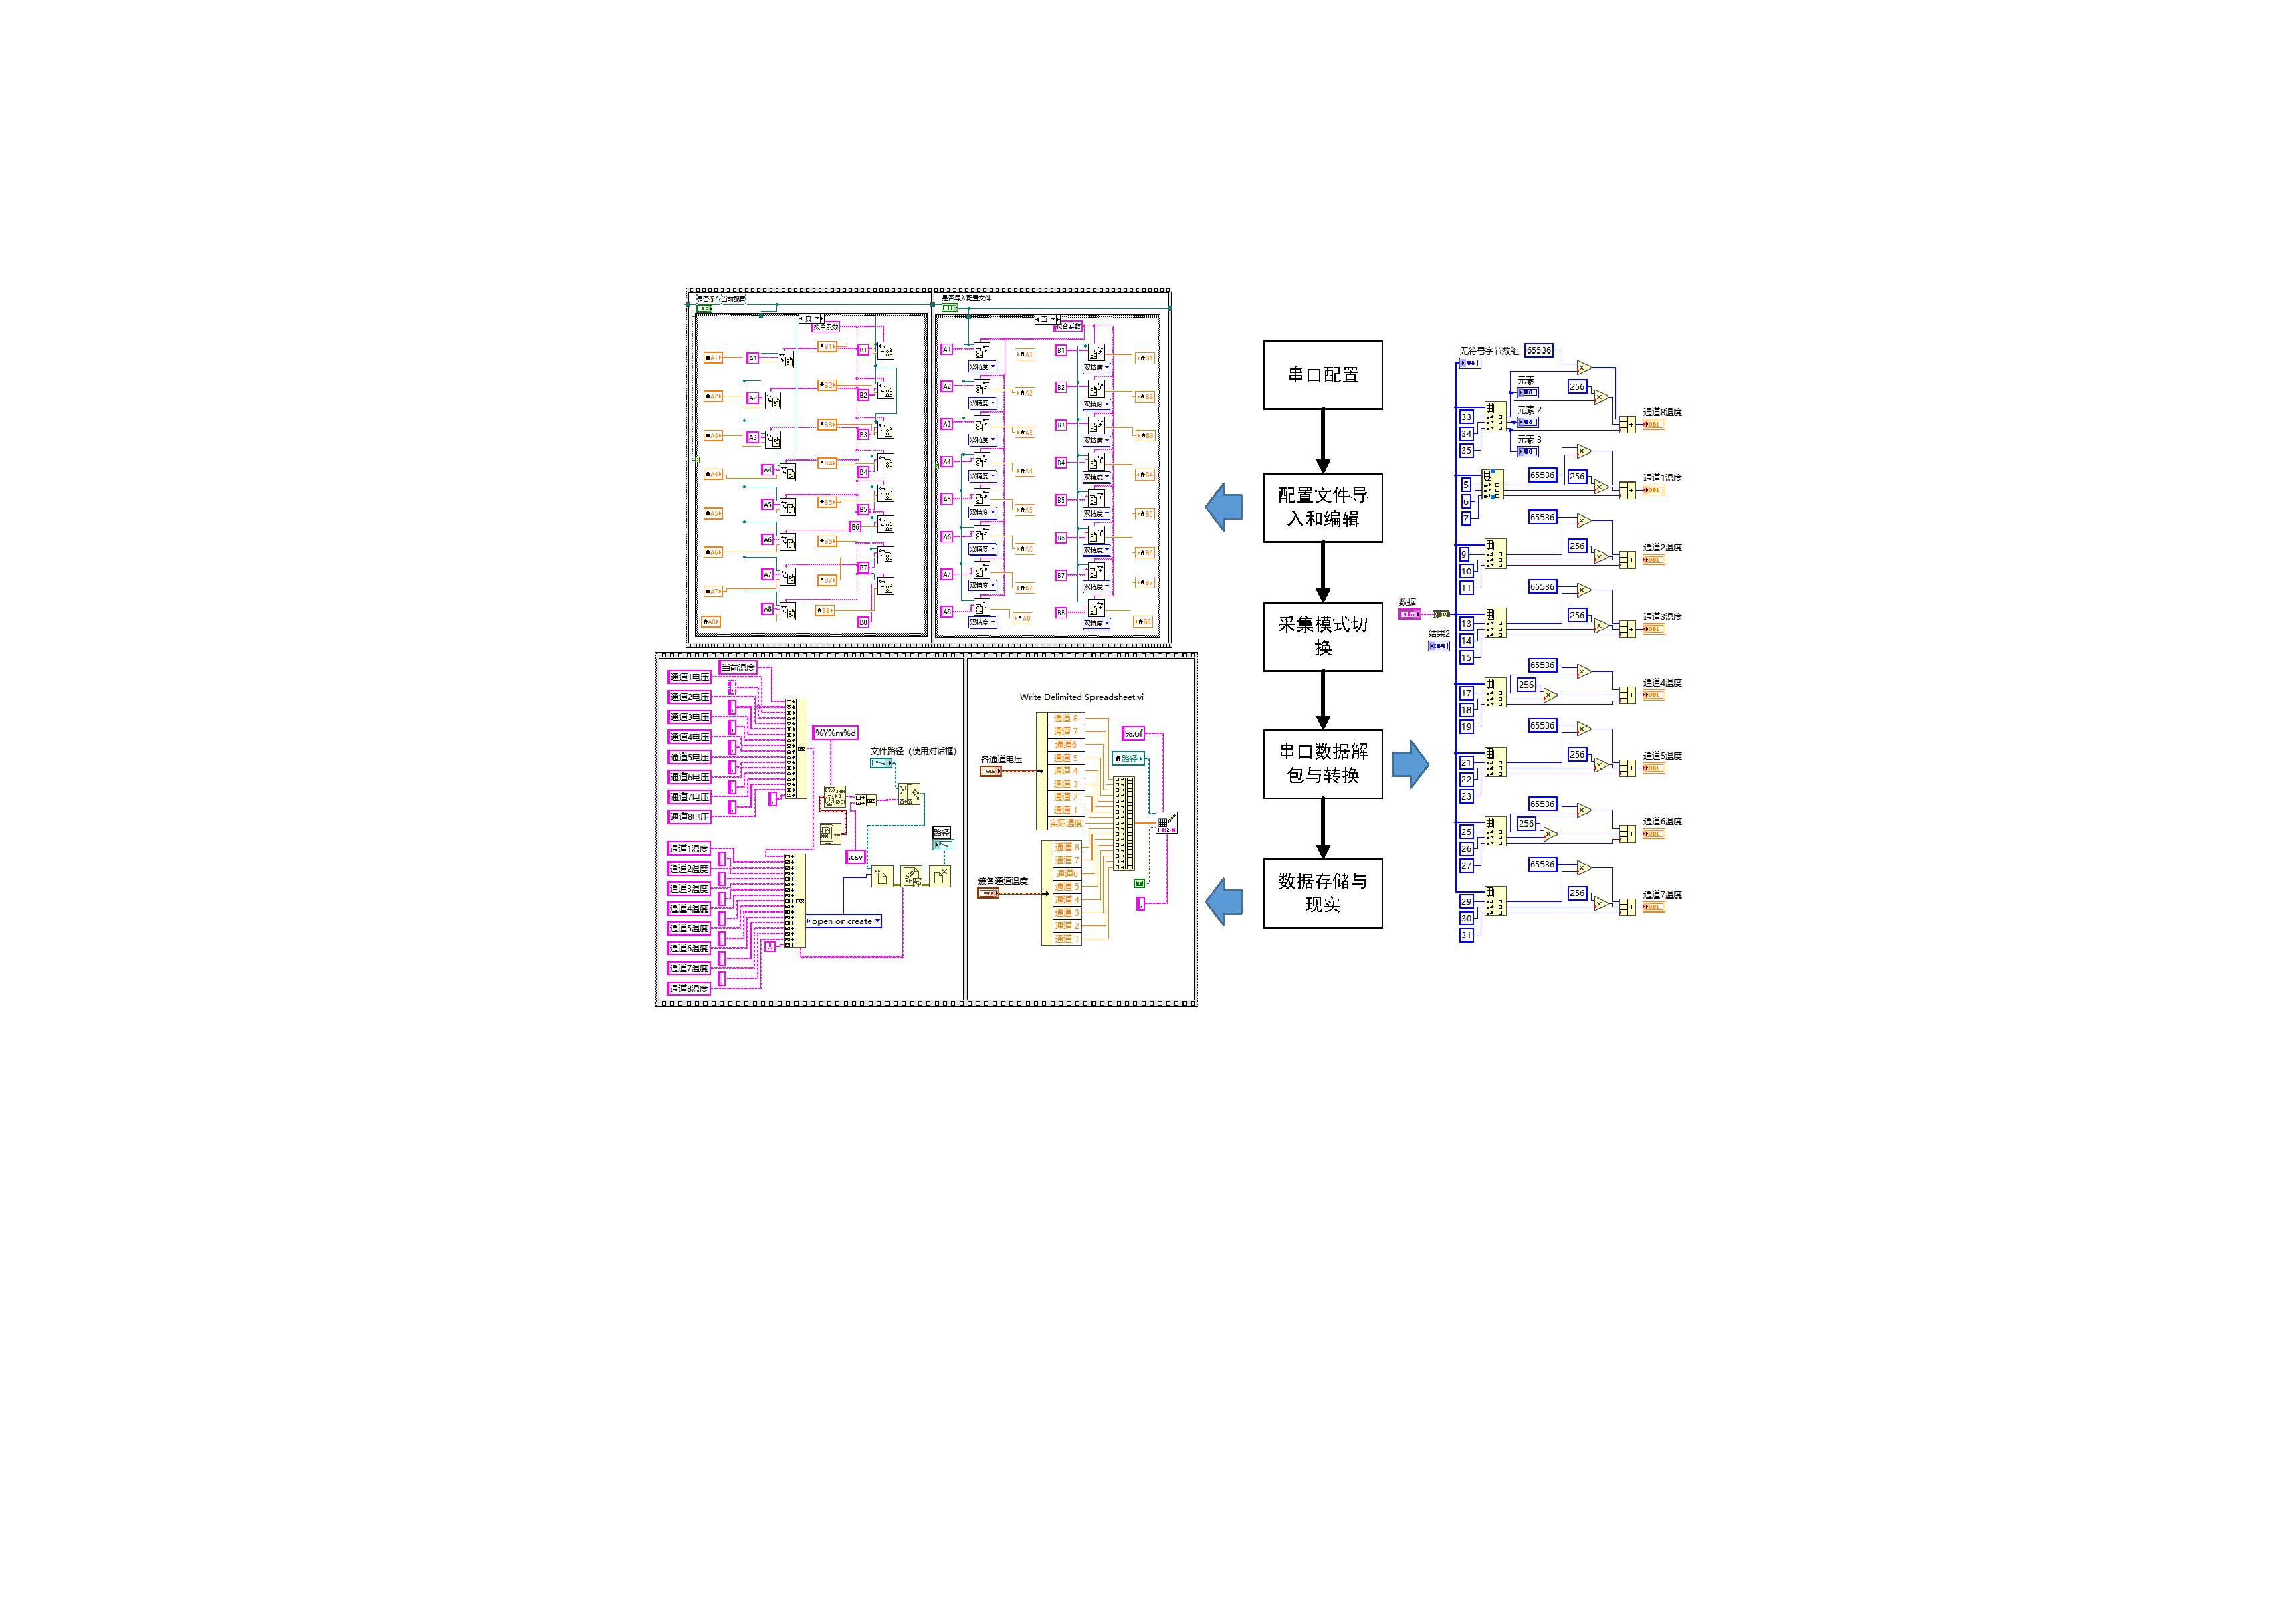
\includegraphics[width=14cm]{fig/3-fig/上位机程序示意图.pdf}
    \caption{上位机程序示意图}
    \label{fig:上位机程序示意图}
\end{figure}

程序的面向用户界面如图\ref{fig:温度测量上位机前面板}所示:
\begin{figure}[htb]
    \centering
    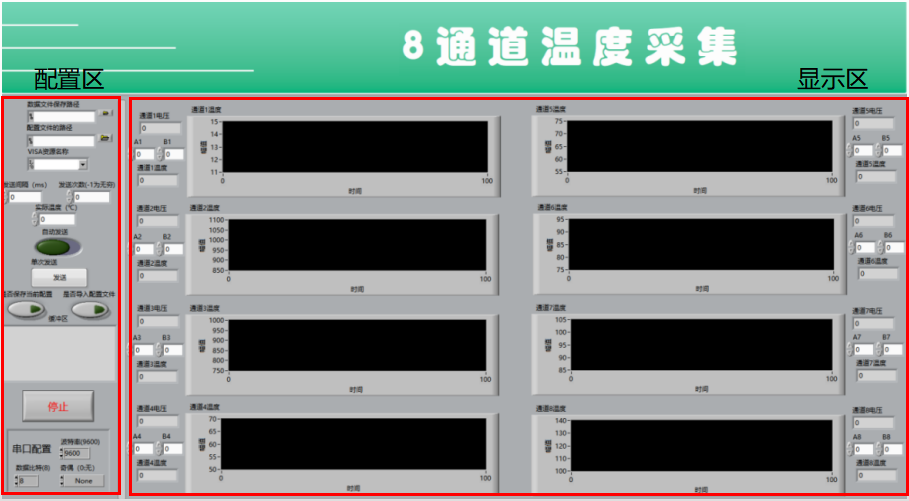
\includegraphics[width=14cm]{fig/3-fig/温度采集上位机前面板.png}
    \caption{温度测量上位机前面板}
    \label{fig:温度测量上位机前面板}
\end{figure}

图\ref{fig:温度测量上位机前面板}分为两个部分:中间的显示区和左侧的配置区。显示区可见8个通道当前的标定系数,以及温度的实时测量值,并且过去一段时间内的温度测量值的变化趋势则会以曲线的形式显示,用户界面的左列配置区可进行以下参数的设定:
\begin{enumerate}
    \item 数据文件保存路径:选择测量数据保存的文件夹路径,程序会自动在该文件夹下产生.csv文件,文件的命名格式为年月日,如20210129。
    \item 配置文件的路径:选择配置文件路径,上位机软件会根据该配置文件里的系数计算温度值,配置文件通常由程序自带的标定拟合功能产生。
    \item 自动发送:自动采集模式与手动采集模式的选择开关,若为自动采集模式,则根据“发送间隔”和“发送次数”两个参数,每隔一段时间进行一次采集,达到设定的采集次数之后程序停止;若为手动采集模式则每次单击“发送”按钮后进行一次采集。
    \item 发送间隔:自动发送模式下,每次发送采集命令之间的时间间隔。
    \item 发送次数:自动发送模式下,发送采集命令的总次数(即采集次数),-1为无穷次。
    \item 实际温度:用于记录当前的实际温度,会在产生的.csv文件中有记录,该项主要用于系统标定时。
    \item 串口配置:设置串口的波特率、数据比特位宽以及奇偶校验位。
  \end{enumerate}

\subsection{标定过程及结果}
基于PT100电阻的多通道温度测量系统标定过程如图\ref{fig:标定示意图}所示,在中空的热沉中灌导热系数较好的油,并在热沉下放置半导体制冷片,半导体制冷片下方放置散热片,两者接触面均匀涂抹导热硅脂,其余位置用黑色保温棉包裹,将待标定的PT100温度传感器捆绑在一起,减少温度不均性带来的误差。使用TCM-X107数字温控模块控制半导体制冷片,并在\(16^{\circ} \mathrm{C} \sim 26^{\circ} \mathrm{C}\)范围内取定几个温度点作为标定点,采用高精度温度传感器T520进行标定,每个标定点待温度稳定之后,以0.5Hz的采样频率,采集一百个数据,去除最大值和最小值之后,以这98个点的平均值作为待标定数据。
  \begin{figure}[htb]
    \centering
    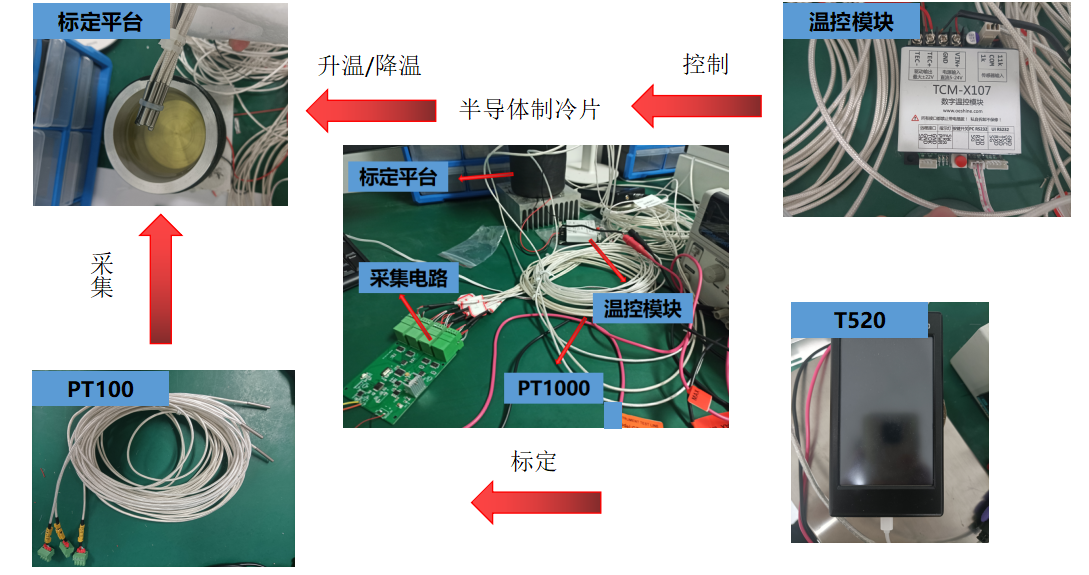
\includegraphics[width=12cm]{fig/3-fig/温度测量系统标定示意图.jpg}
    \caption{标定示意图}
    \label{fig:标定示意图}
\end{figure}

标定程序界面如图\ref{fig:标定程序用户界面}所示,红色的点为8个通道采集到的离散的温度数据,蓝色曲线为标定程序输出的拟合曲线,程序会自动根据标定结果生成.ini配置文件,供测量系统上位机使用。
\begin{figure}[htb]
    \centering
    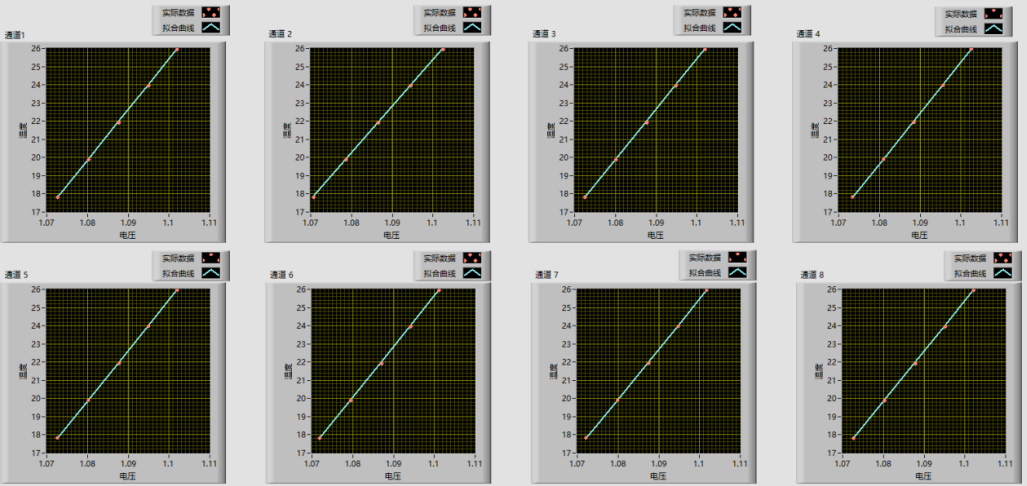
\includegraphics[width=13cm]{fig/3-fig/标定程序前面板.jpg}
    \caption{标定程序用户界面}
    \label{fig:标定程序用户界面}
\end{figure}

部分标定结果如表\ref{tab:标定误差值}所示,在所有标定结果中最大误差为$0.038^{\circ} \mathrm{C}$,部分点误差大于$0.01^{\circ} \mathrm{C}$,绝大部分点误差小于$0.01^{\circ} \mathrm{C}$,并且8个通道的拟合优度$R^2$值都大于0.9999。
\begin{table}[H]
    \centering
    \caption{标定误差值}
    \label{tab:标定误差值}
    \resizebox{\textwidth}{14mm}{
    \begin{tabular}{ccccccccc}
        \hline
                      &   通道1/$^{\circ} \mathrm{C}$ & 通道2/$^{\circ} \mathrm{C}$ & 通道3/$^{\circ} \mathrm{C}$ & 通道4/$^{\circ} \mathrm{C}$ & 通道5/$^{\circ} \mathrm{C}$ & 通道6/$^{\circ} \mathrm{C}$ & 通道7/$^{\circ} \mathrm{C}$ & 通道8/$^{\circ} \mathrm{C}$ \\ \hline
    17.804$^{\circ} \mathrm{C}$ & -0.0037 & 0.0037 & 0.0176 & 0.0072  & -0.0112 & 0.0101  & -0.0192 & -0.0279  \\ \hline
    19.879$^{\circ} \mathrm{C}$ & 0.0008  & 0.0142 & 0.0209 & 0.0075  & 0.0030  & 0.0161  & -0.0052 & -0.0127  \\ \hline
    21.944$^{\circ} \mathrm{C}$ & -0.0042 & 0.0022 & 0.0051 & -0.0037 & 0.0008  & -0.0015 & -0.0029 & -0.0030  \\ \hline
    24.047$^{\circ} \mathrm{C}$ & 0.0008  & 0.0049 & 0.0123 & 0.0068  & 0.0033  & 0.0039  & -0.0074 & -0.0169  \\ \hline
    26.107$^{\circ} \mathrm{C}$ & 0.0071  & 0.0017 & 0.0173 & 0.0116  & 0.0016  & 0.0078  & -0.0108 & -0.0162  \\ \hline
    \end{tabular}}
  \end{table}
\section{气压测量系统}
气压测量系统采用美国GE Druck公司PACE1000传感器,如图\ref{fig:PACE1000气压传感器}所示,精度为4Pa,能够支持最小值/最大值/平均值显示,长期稳定性高达0.01\%Rdg每年,带有可选择的图形显示以及数据存储功能\cite{PACE1000}。
\begin{figure}[htb]
    \centering
    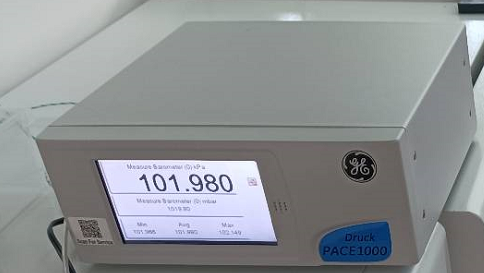
\includegraphics[width=8cm]{fig/3-fig/PACE1000气压传感器.jpg}
    \caption{PACE1000气压传感器}
    \label{fig:PACE1000气压传感器}
\end{figure}

\section{补偿系统总体方案}
补偿系统总体包括一套单轴双频激光干涉仪测量系统、隔震光学平台、温度测量模块和压力传感器四个部分,单轴双频激光干涉仪测量系统所用的的激光器为Agilent公司的5517A双频激光器,其名义波长为632.991354nm,1小时内的激光波长稳定性为0.002ppm,在90mm光程下,激光器自带的波长误差约为0.18nm,实物图如图\ref{fig:激光器实物图}所示。
\begin{figure}[htb]
    \centering
    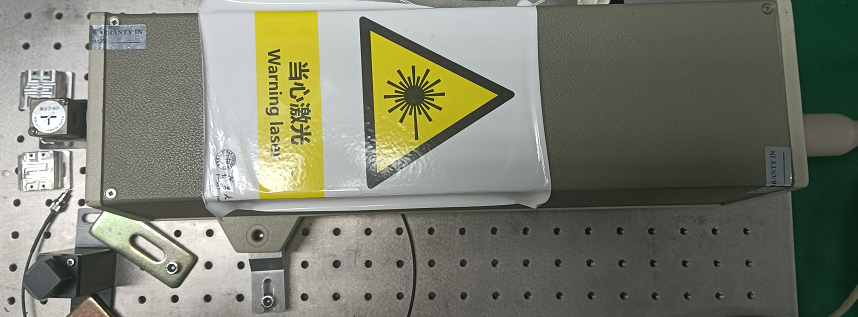
\includegraphics[width=10cm]{fig/3-fig/激光器实物图.png}
    \caption{激光器实物图}
    \label{fig:激光器实物图}
\end{figure}

干涉仪的光学细分为4,为了减小温度对材料热胀冷缩的影响,本文工作所用的干涉仪为实验室自制,使用光学元件直接粘接制成,并无任何的金属外壳,并且将底座粘接在微晶玻璃上,如图\ref{fig:干涉仪实物图}所示,微晶玻璃为德国肖特SCHOTT公司Class0级的微晶玻璃,其热膨胀系数小于$2\times 10^{-8}$,对于本文采用的测量臂长度为45mm和90mm的两套单轴双频激光干涉仪,当温度变化$1^{\circ} \mathrm{C}$时,由于材料热胀冷缩引入的误差不会超过1.8nm,相对于环境误差而言,这是可以忽略不计的。
\begin{figure}[htb]
    \centering
    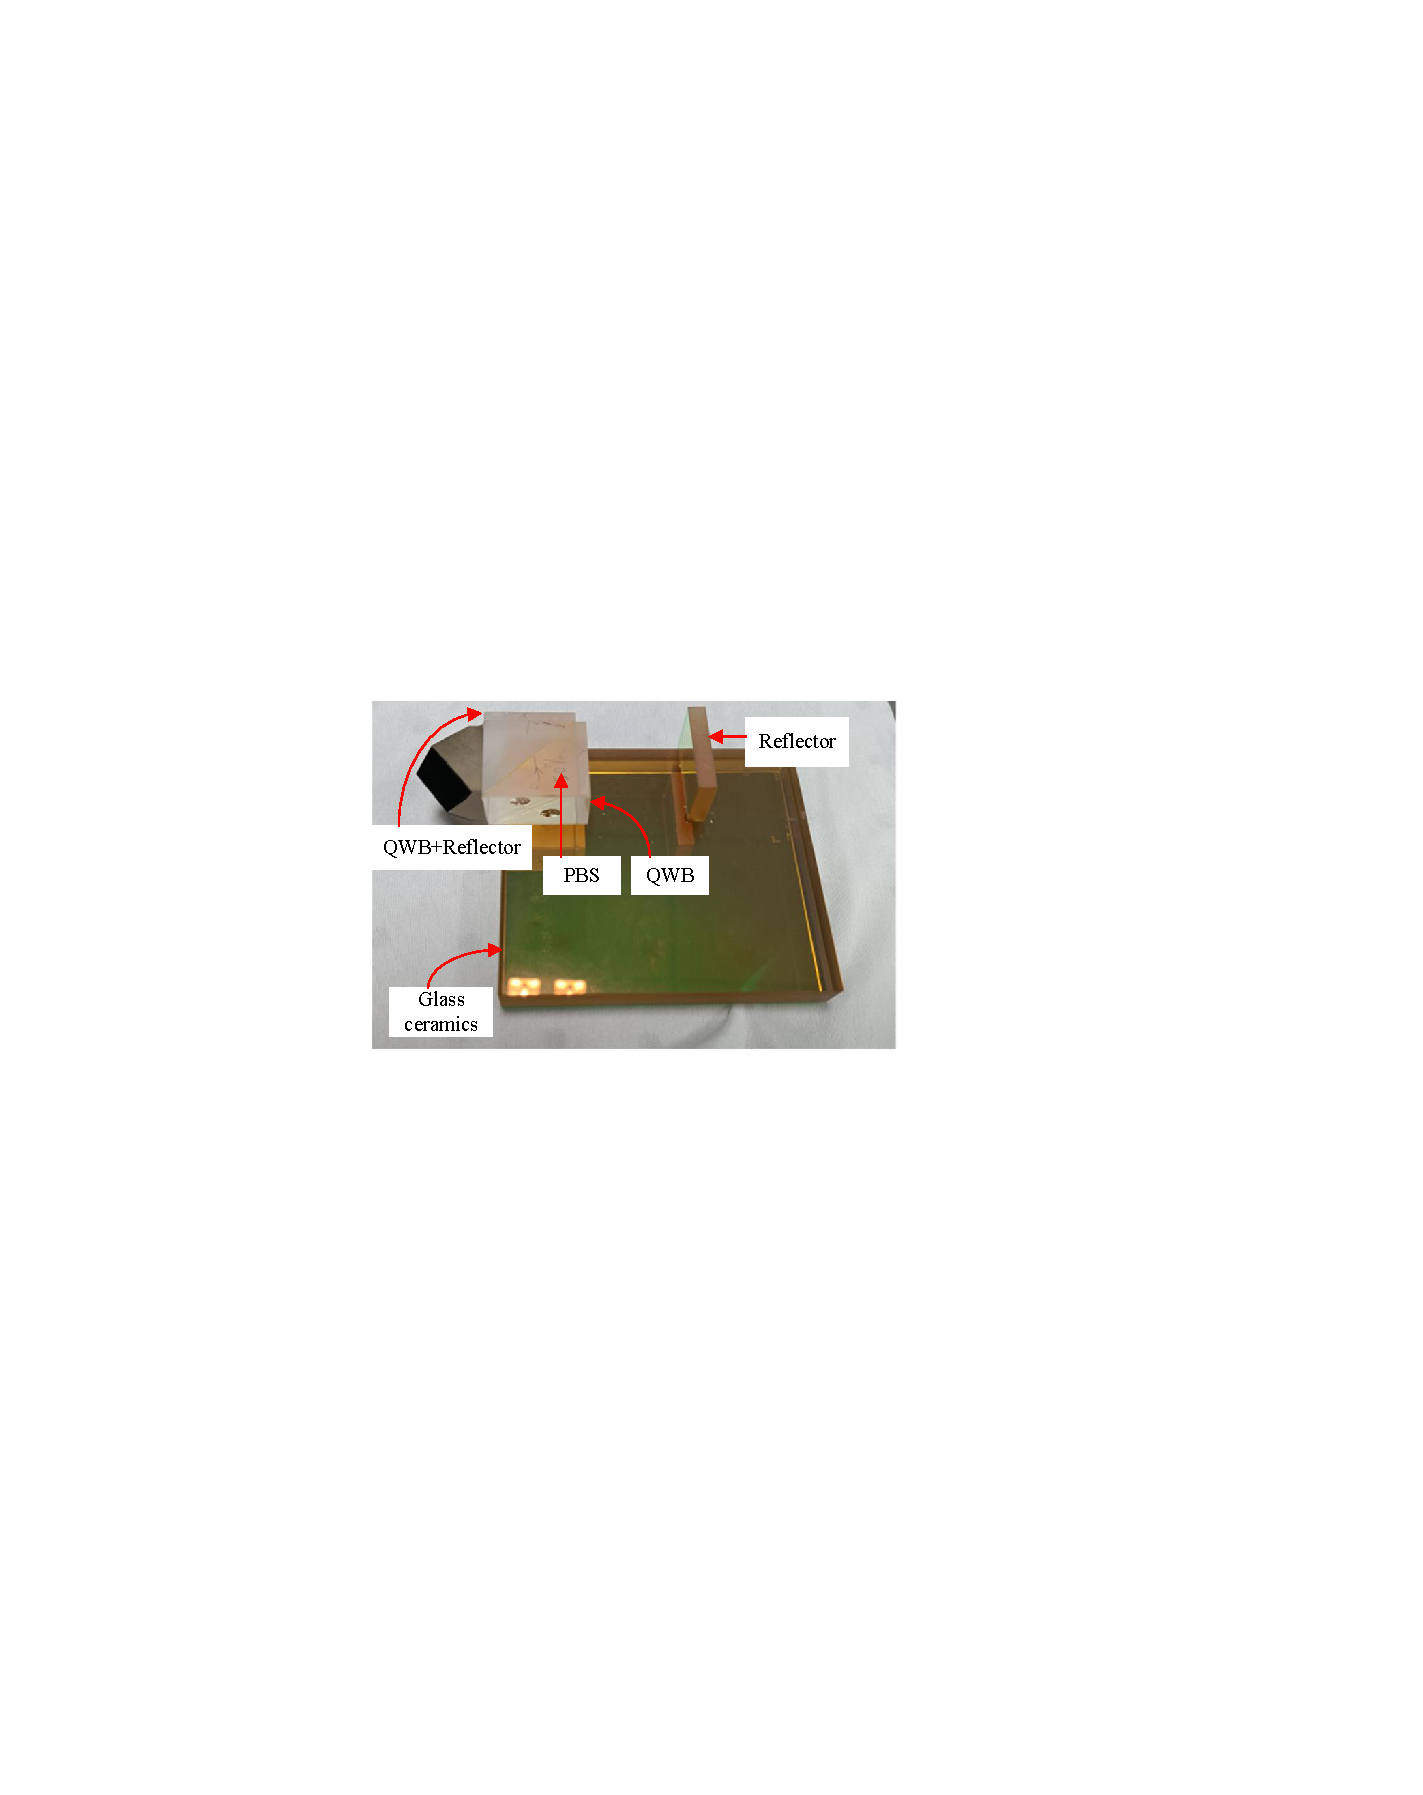
\includegraphics[width=8cm]{fig/3-fig/干涉仪实物图.pdf}
    \caption{干涉仪实物图}
    \label{fig:干涉仪实物图}
\end{figure}

系统中使用的信号采集卡为上海拍频光电科技有限公司的ELIB0306A三轴外差信号解调器,如图\ref{fig:信号采集卡实物图}所示,电子细分为32,信号采样率为10MHz,最多支持3个通道同时采样\cite{信号处理卡}。根据式\eqref{eq:分辨率与细分的关系}可知,该单轴双频激光干涉仪系统的分辨率约为4.9nm,这也再次说明了,上述的激光器自带的波长误差以及微晶玻璃热胀冷缩的影响可以忽略不计。
\begin{figure}[htb]
    \centering
    \includegraphics[width=8cm]{fig/3-fig/信号采集卡实物图.jpg}
    \caption{信号采集卡实物图}
    \label{fig:信号采集卡实物图}
\end{figure}

\section{实验方案及其改进}
在本文所述工作中,为了能够更精准地测量到干涉仪的环境误差,在实验方案上进行了多次改进:
\begin{enumerate}
    \item 实验设备方面:将干涉仪从常见的带有金属外壳的干涉仪改变为将各光学器件直接粘接制成的干涉仪以减少热胀冷缩带来的误差。
    \item 实验变量方面:从仅测量温度变为温度气压同时测量,虽然温度是影响干涉仪环境误差的最重要因素,但是仅仅对温度变量进行补偿无法满足精度要求,所以增加气压变量的补偿。
    \item 实验环境方面:从不采取任何隔震措施变为使用带有气浮隔震功能的光学平台,以减小震动带来的误差干扰;从有直接热源控制温度测量环境误差变为完全使用环境温度的自然变化来测量环境误差,以消除热源带来的误差干扰。
    \item 实验方法方面:从单一实验变为对比实验,由式\eqref{eq:环境误差公式}可以看出,干涉仪的环境误差是跟测量臂长度成正比的,所以衡量干涉仪环境误差补偿是否精准的方式为判断不同测量臂长度下补偿后残差是否一致,一致即为精准补偿,所以设立了45mm和90mm两种测量臂长度的实验组。
  \end{enumerate}
\subsection{实验设备改进}
传统的干涉仪如图\ref{fig:带金属外壳的干涉仪}所示,光学元器件粘贴在金属底座上,并且置有金属外壳。采用该种干涉仪的实验装置图如图\ref{fig:实验系统图-带外壳干涉仪}所示,进行零位测量得到的测量数据如图\ref{fig:带外壳干涉仪的实验数据}所示。可以看出在7h的测量时间里温度变化了约$0.6^{\circ} \mathrm{C}$,但是干涉仪测出的位移却达到了3000nm,这个数量级的误差明显超出环境误差的范畴。并且由图\ref{fig:折射率-温度}可以看出,温度升高,空气折射率是降低的,带入\eqref{eq:环境误差公式}可知,由环境误差导致的干涉仪测量值应该是个负数,而实际测量值却是一个正数,所以大致可以断定是由于温度升高,导致干涉仪的金属底座以及被测物底座受热膨胀而导致出现正向位移误差值。所以后续采用如图\ref{fig:干涉仪实物图}所示的干涉仪,将PBS、反射镜、玻片等用光学胶直接粘接制成,并且干涉仪和被测物(反射镜)都直接粘在微晶玻璃上,以减小热胀冷缩带来的误差。
\begin{figure}[htb]
    \centering
    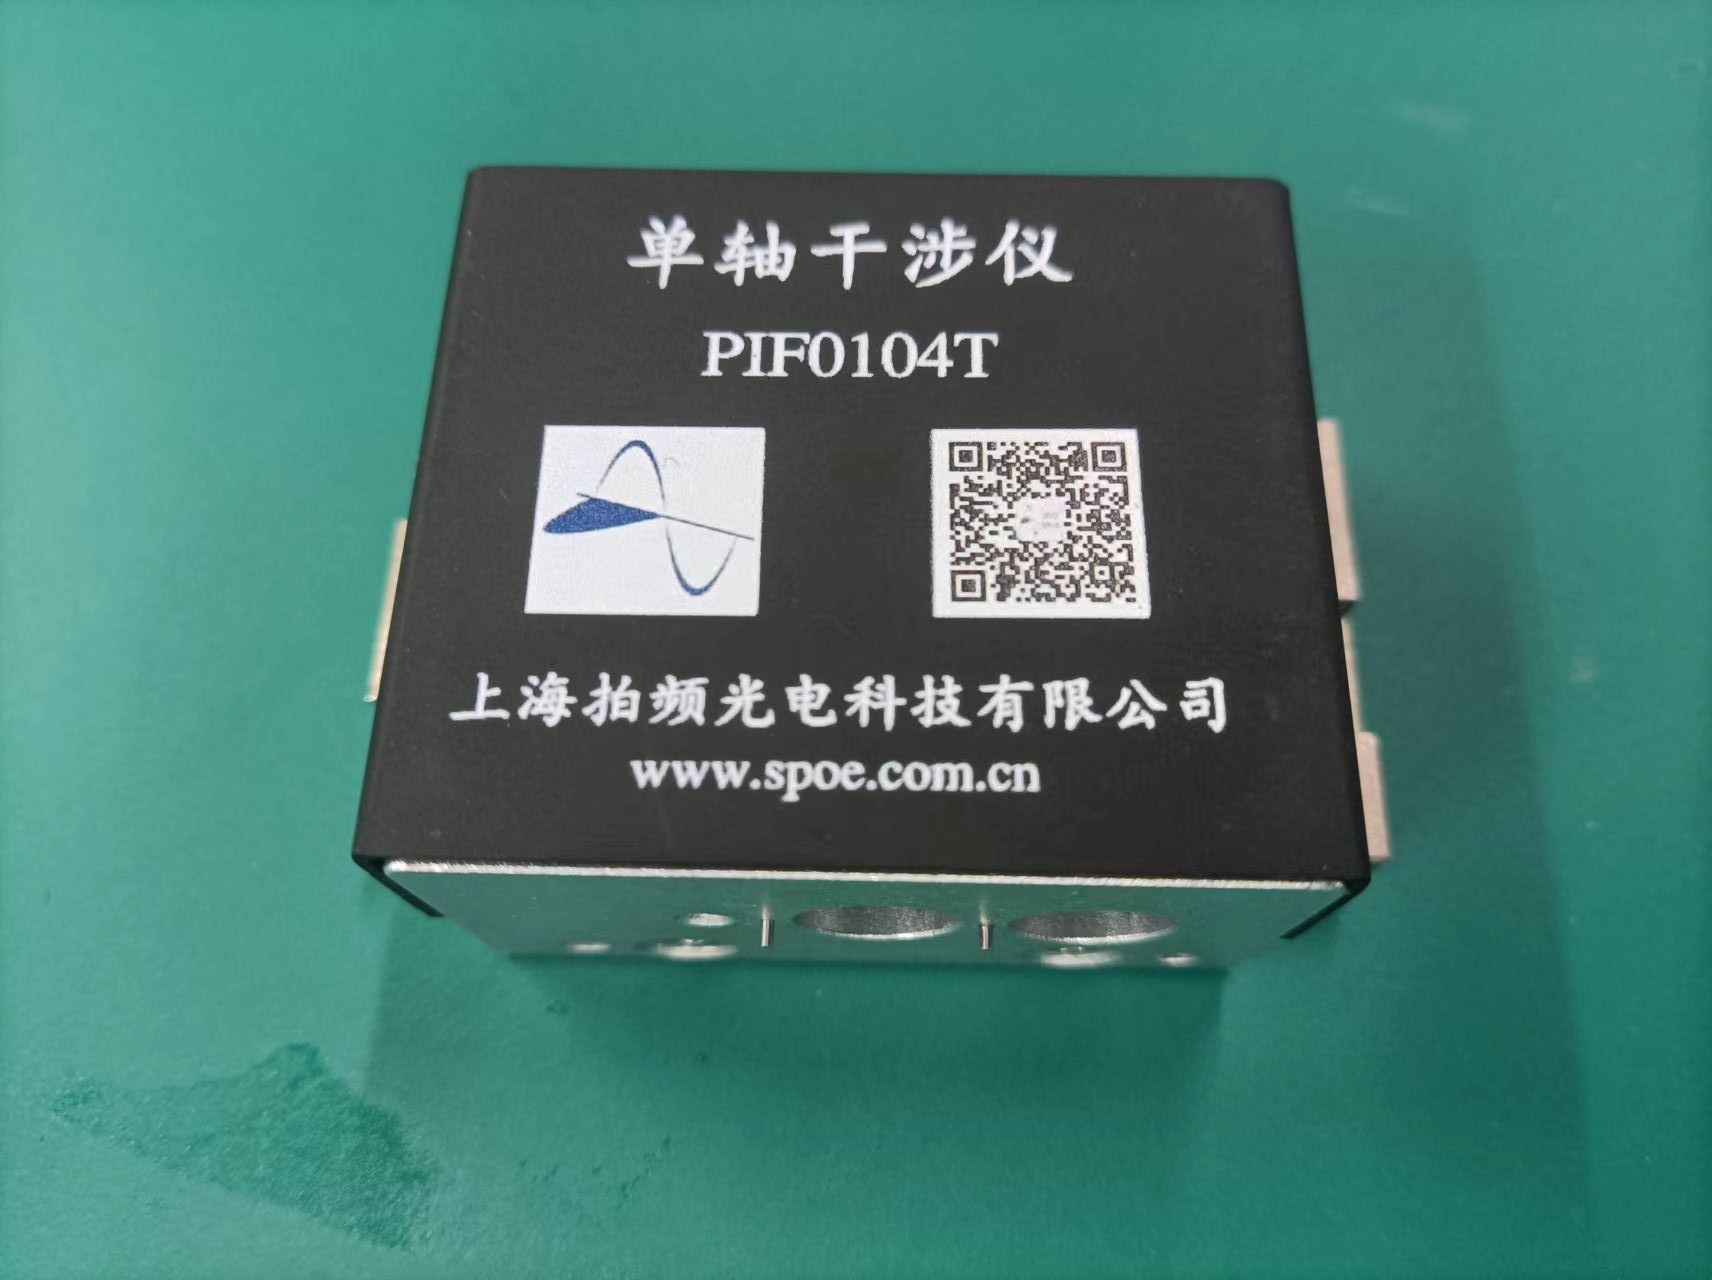
\includegraphics[width=6cm]{fig/3-fig/带金属外壳的干涉仪.jpg}
    \caption{带金属外壳的干涉仪}
    \label{fig:带金属外壳的干涉仪}
\end{figure}
\begin{figure}[htb]
    \centering
    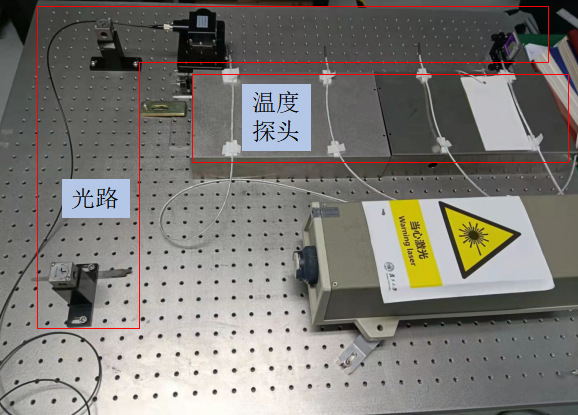
\includegraphics[width=8cm]{fig/3-fig/实验系统图-带外壳干涉仪.jpg}
    \caption{实验系统图-带外壳干涉仪}
    \label{fig:实验系统图-带外壳干涉仪}
\end{figure}
\begin{figure}[htb]
    \centering
    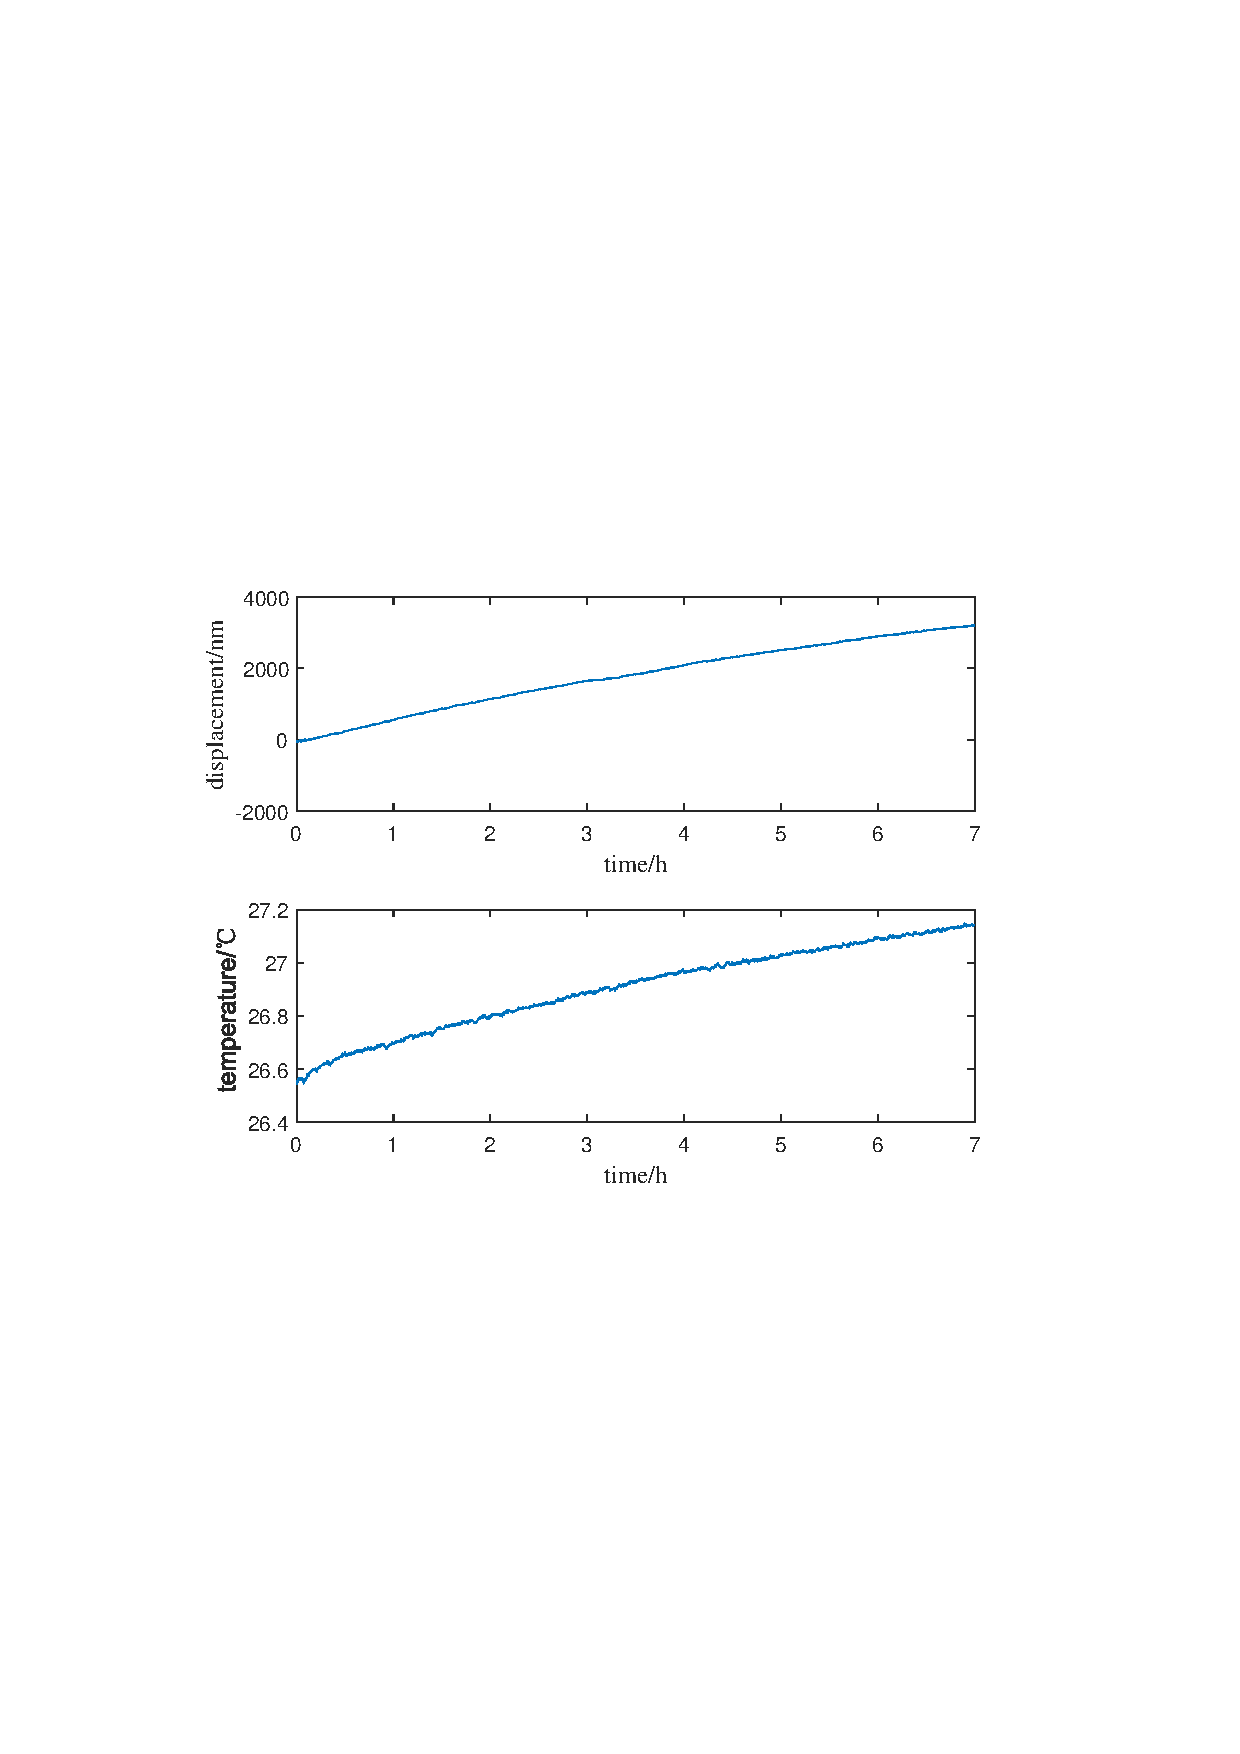
\includegraphics[width=12cm]{fig/3-fig/实验数据-带外壳的干涉仪.pdf}
    \caption{带外壳干涉仪的实验数据}
    \label{fig:带外壳干涉仪的实验数据}
\end{figure}

\subsection{实验变量改进}
将干涉仪和被测物体粘接在微晶玻璃后的实验装置如图\ref{fig:实验系统图-带微晶玻璃}所示,如前文所述,此时由于热胀冷缩带来的误差是可以忽略不计的。进行零位测量得到的测量数据如图\ref{fig:实验数据-带微晶玻璃}所示,从图中可以看出约480nm的环境误差,如果仅仅对温度这一单一变量进行误差补偿,残留误差仍有约180nm,虽然补偿了约$60\%$的误差,但是残余值仍不可以忽略,所以需要增加实验变量,即对气压也进行补偿。
\begin{figure}[htb]
  \centering
  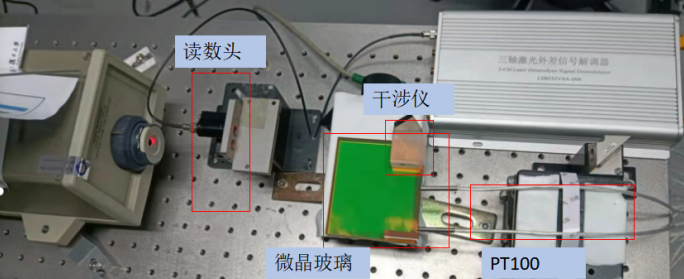
\includegraphics[width=12cm]{fig/3-fig/实验系统图-带微晶玻璃.jpg}
  \caption{实验系统图-带微晶玻璃}
  \label{fig:实验系统图-带微晶玻璃}
\end{figure}
\begin{figure}[htb]
  \centering
  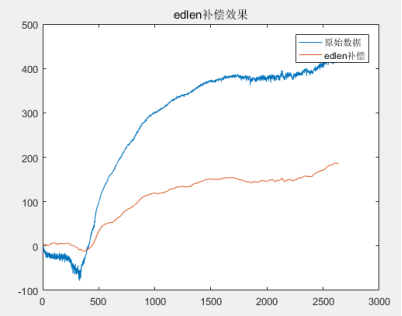
\includegraphics[width=7cm]{fig/3-fig/实验数据-带微晶玻璃.jpg}
  \caption{实验数据-带微晶玻璃}
  \label{fig:实验数据-带微晶玻璃}
\end{figure}

\subsection{实验环境改进}
\label{section:实验环境改进}
带温控箱的实验装置图如图\ref{fig:带温控箱的实验装置图}所示,图\ref{fig:实验示意图-带温控箱}为示意图,图\ref{fig:实验系统图-带温控箱}为实物图。
\begin{figure}[htb]
    \centering
    \subfigure[实验示意图-带温控箱]{
      \begin{minipage}[b]{0.80\textwidth}
        \centering
        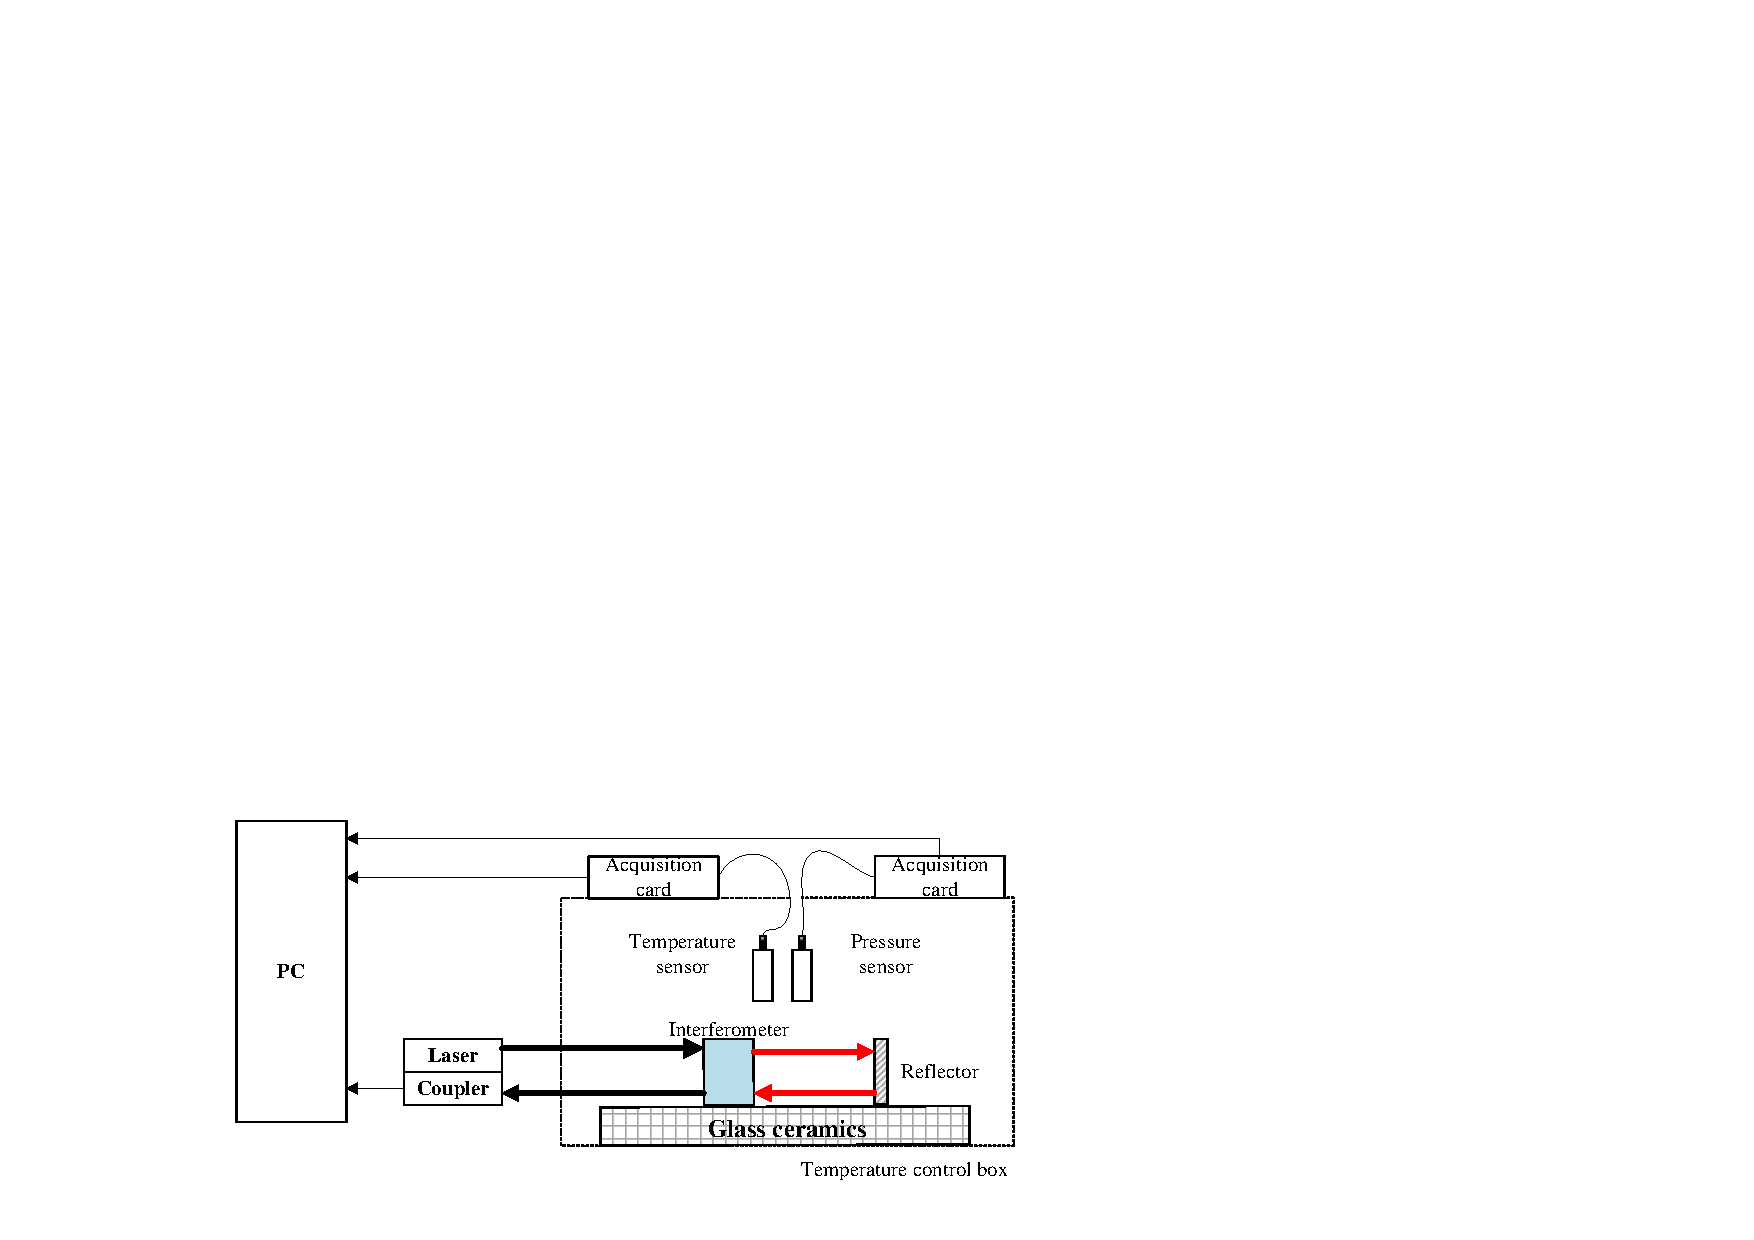
\includegraphics[width=10cm,height=5cm]{fig/3-fig/实验示意图-带温控箱.pdf}
      \end{minipage}
      \label{fig:实验示意图-带温控箱}
    }
    \subfigure[实验系统图-带温控箱]{
      \begin{minipage}[b]{0.80\textwidth}
        \centering
        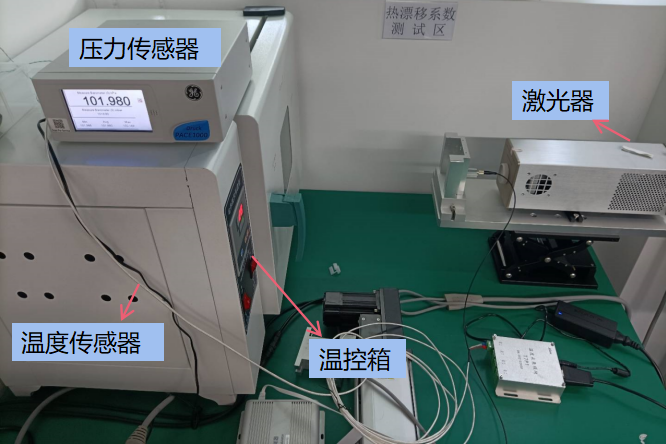
\includegraphics[width=9cm,height=6cm]{fig/3-fig/实验系统图-带温控箱.jpg}
      \end{minipage}
      \label{fig:实验系统图-带温控箱}
    }
    \caption{带温控箱的实验装置图}
    \label{fig:带温控箱的实验装置图}
  \end{figure}
实验数据如图\ref{fig:带温控箱的实验数据}所示,5h的测量时间内,温度变化约为$0.1^{\circ} \mathrm{C}$,气压变化约为0.25kPa,排除了热胀冷缩的影响之后,位移的误差值降到了几十nm级别,属于环境误差的合理范畴。但从图中可以明显看出,相较于平滑的压力曲线,温度曲线有着较多的毛刺,这也使得干涉仪系统的位移测量值也有着较多毛刺,这是由于温控箱工作导致的温度不均匀引起的。所以后续大部分实验采用测量环境温度的自然变化,并且增加气浮功能用于隔震。
\begin{figure}[htb]
    \centering
    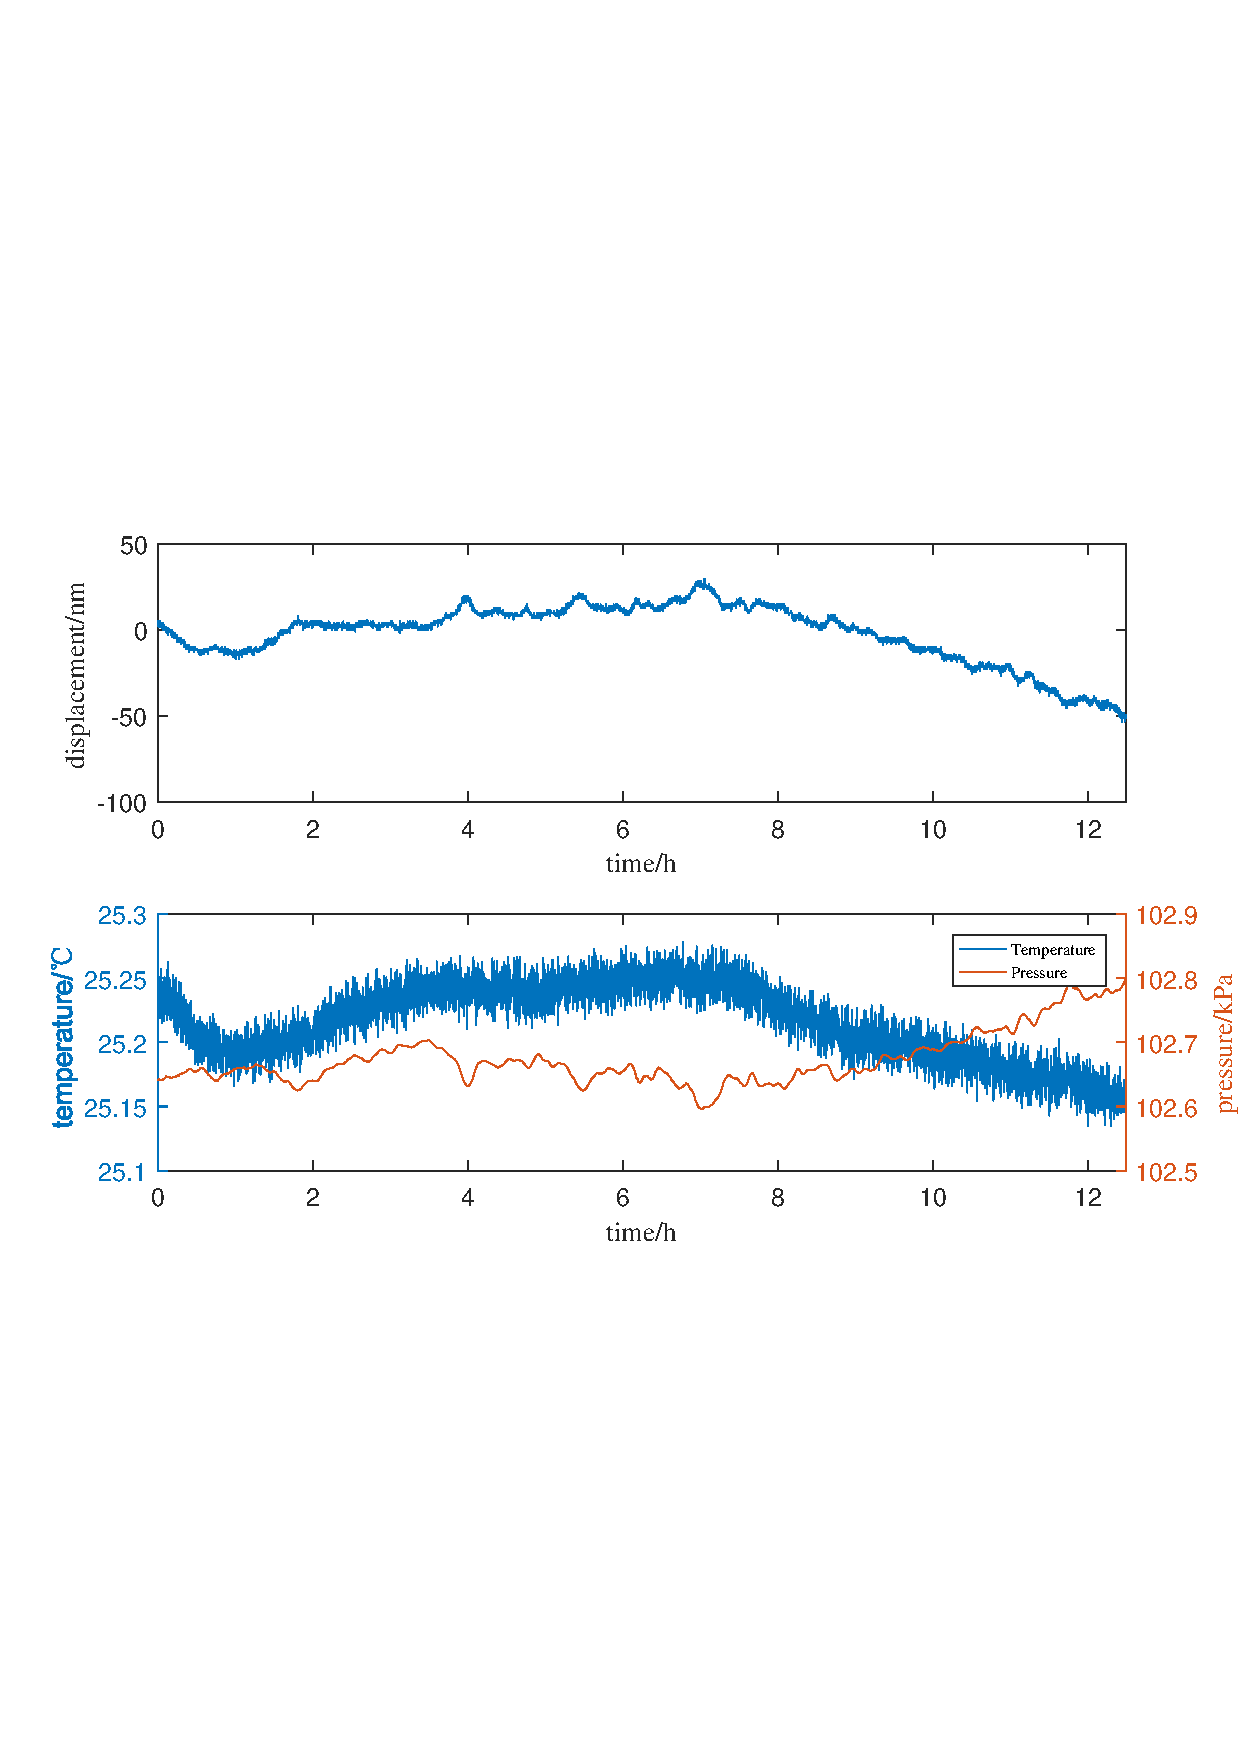
\includegraphics[width=12cm]{fig/3-fig/实验数据-温控箱.pdf}
    \caption{带温控箱的实验数据}
    \label{fig:带温控箱的实验数据}
\end{figure}

\subsection{最终实验方案}
最终实验方案如图\ref{fig:最终实验方案}所示,图\ref{fig:最终实验示意图}为示意图,图\ref{fig:最终实验系统图}为实物图。测量臂长度为45mm和90mm的两套干涉仪都是粘接在微晶玻璃上,并且放置在亚克力罩内,温度传感器探头和压力传感器探头也固定在亚克力罩内。激光器出射的激光经过$50\%$分光镜分成两束强度均匀的光后分别进入两套干涉仪系统,并且经两个光纤耦合器后接入采集板卡。所有光学器件都由卡座固定在光学平台上,并且光学平台开启了气浮功能以减少震动的影响。
\begin{figure}[htb]
    \centering
    \subfigure[最终实验示意图]{
      \begin{minipage}[b]{0.90\textwidth}
        \centering
        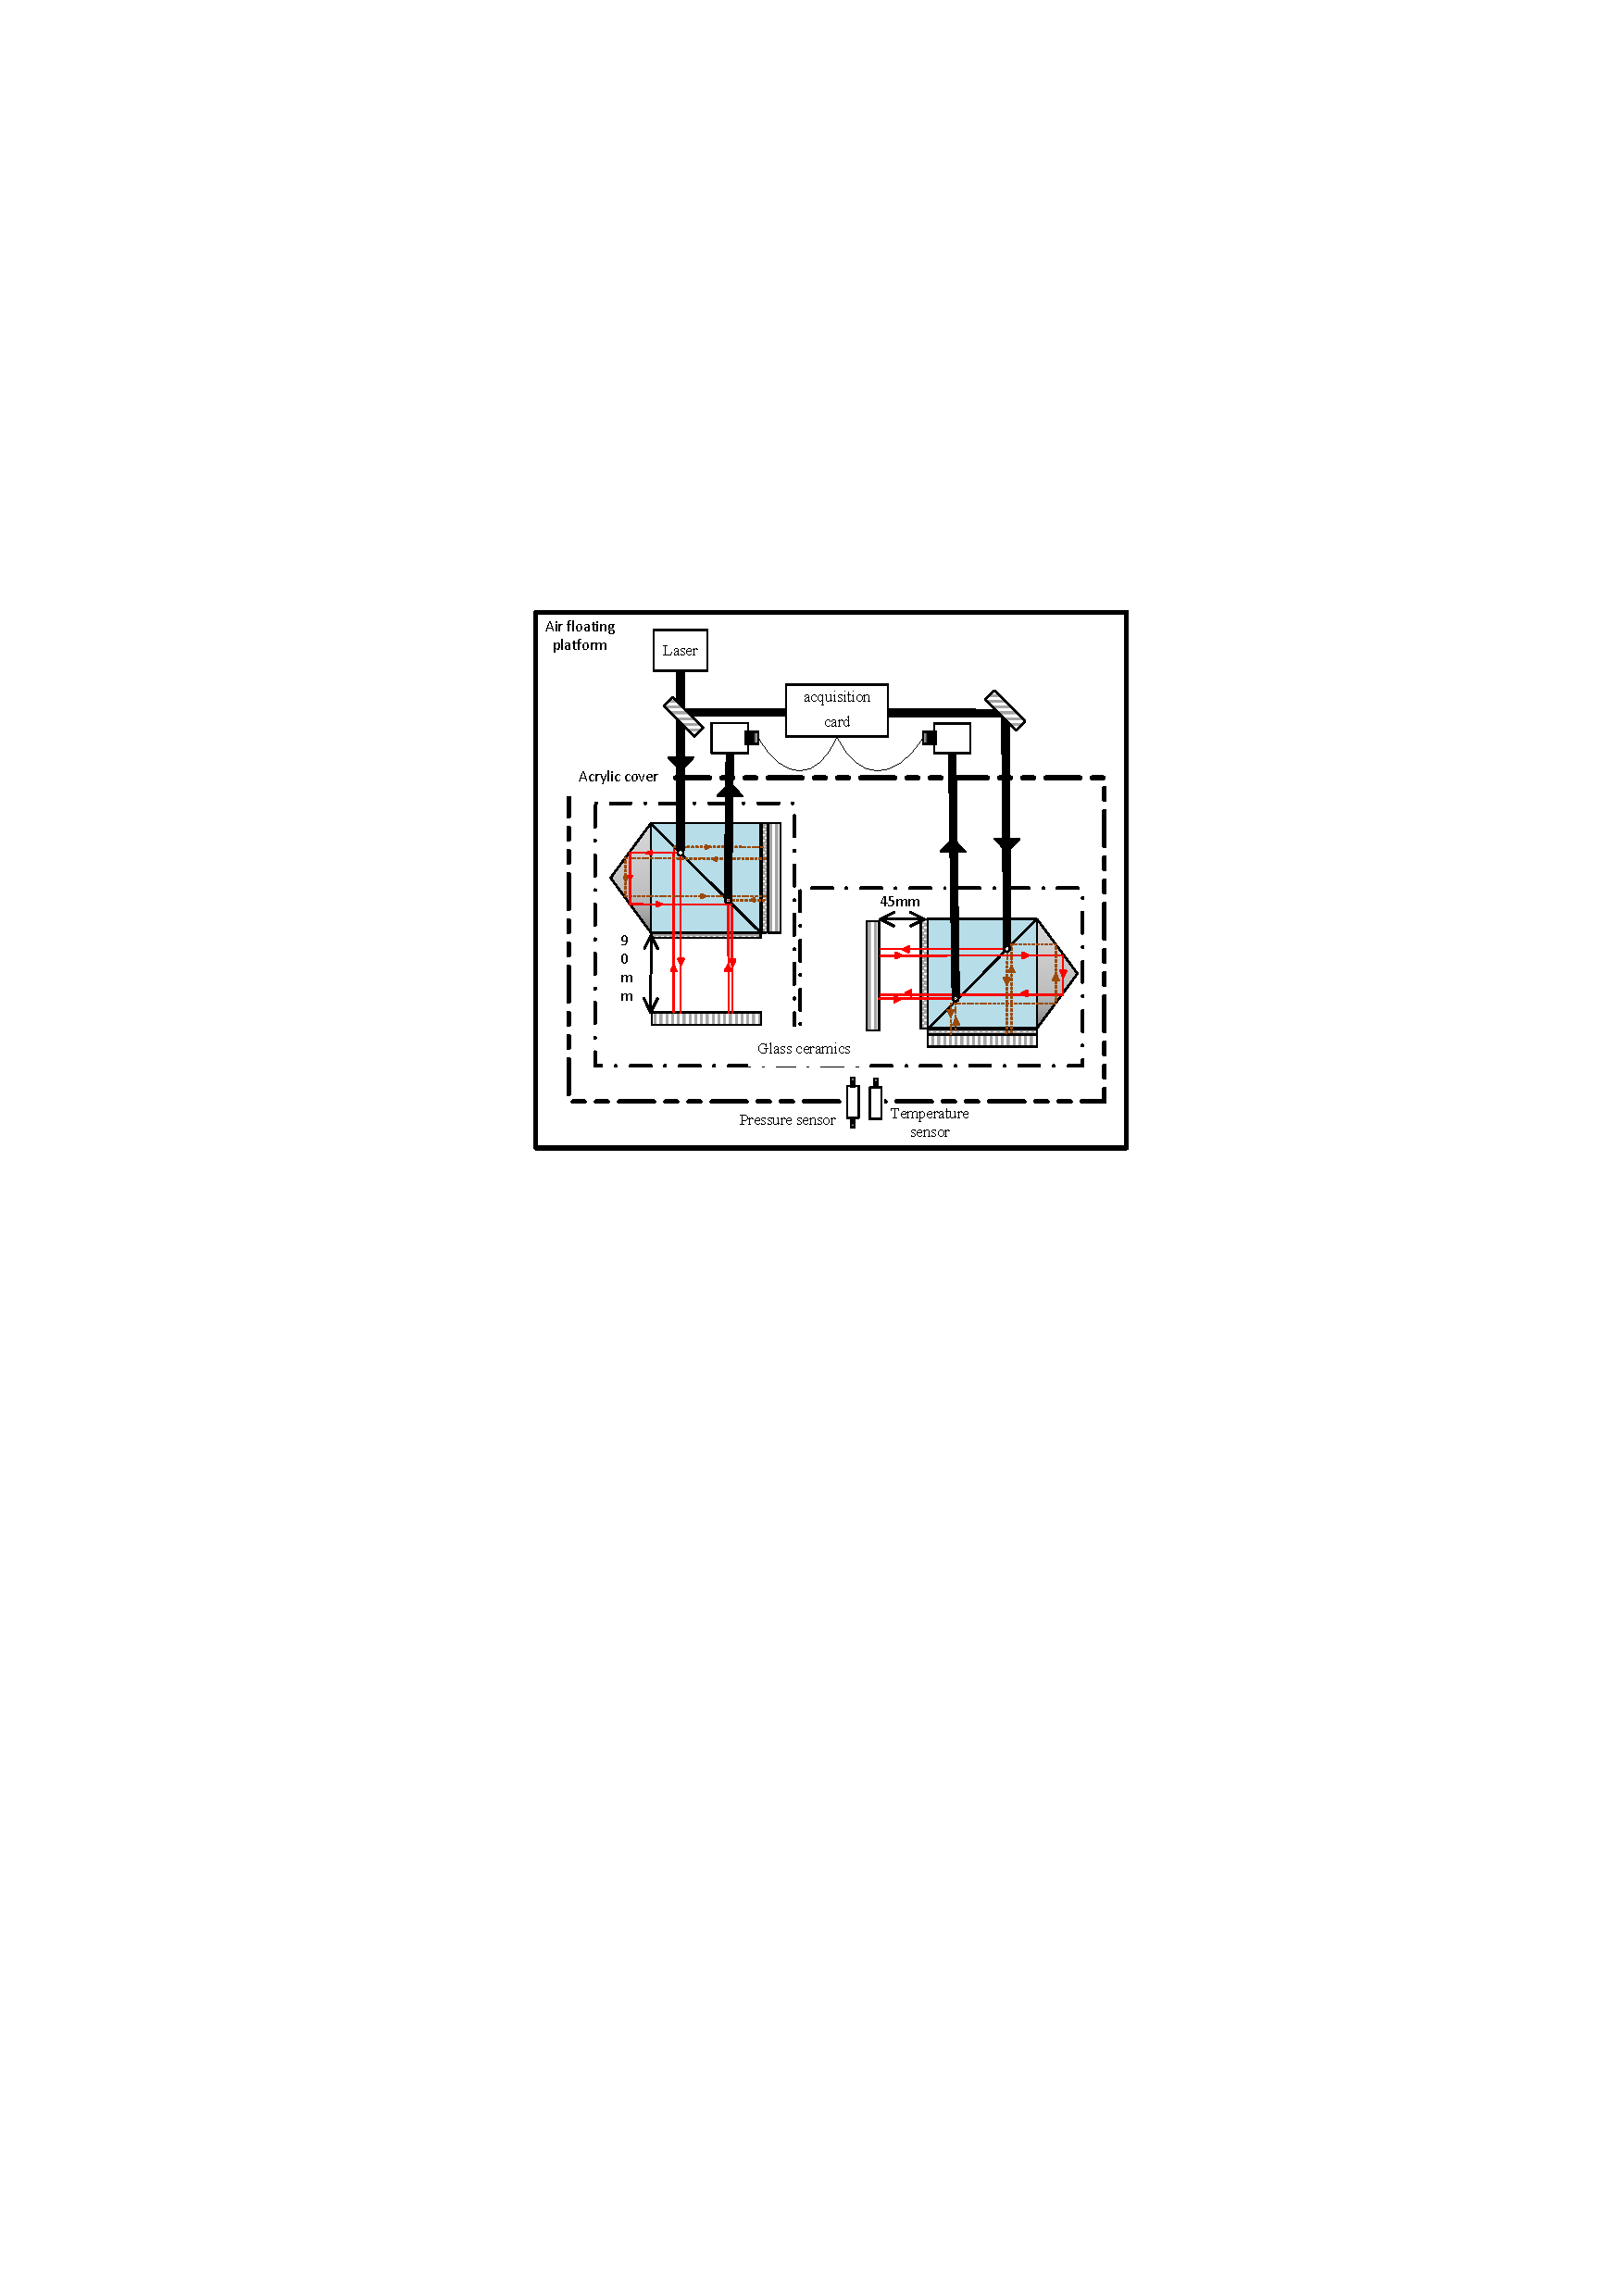
\includegraphics[width=10.5cm,height=7.5cm]{fig/3-fig/最终实验示意图.pdf}
      \end{minipage}
      \label{fig:最终实验示意图}
    }
    \subfigure[最终实验系统图]{
      \begin{minipage}[b]{0.90\textwidth}
        \centering
        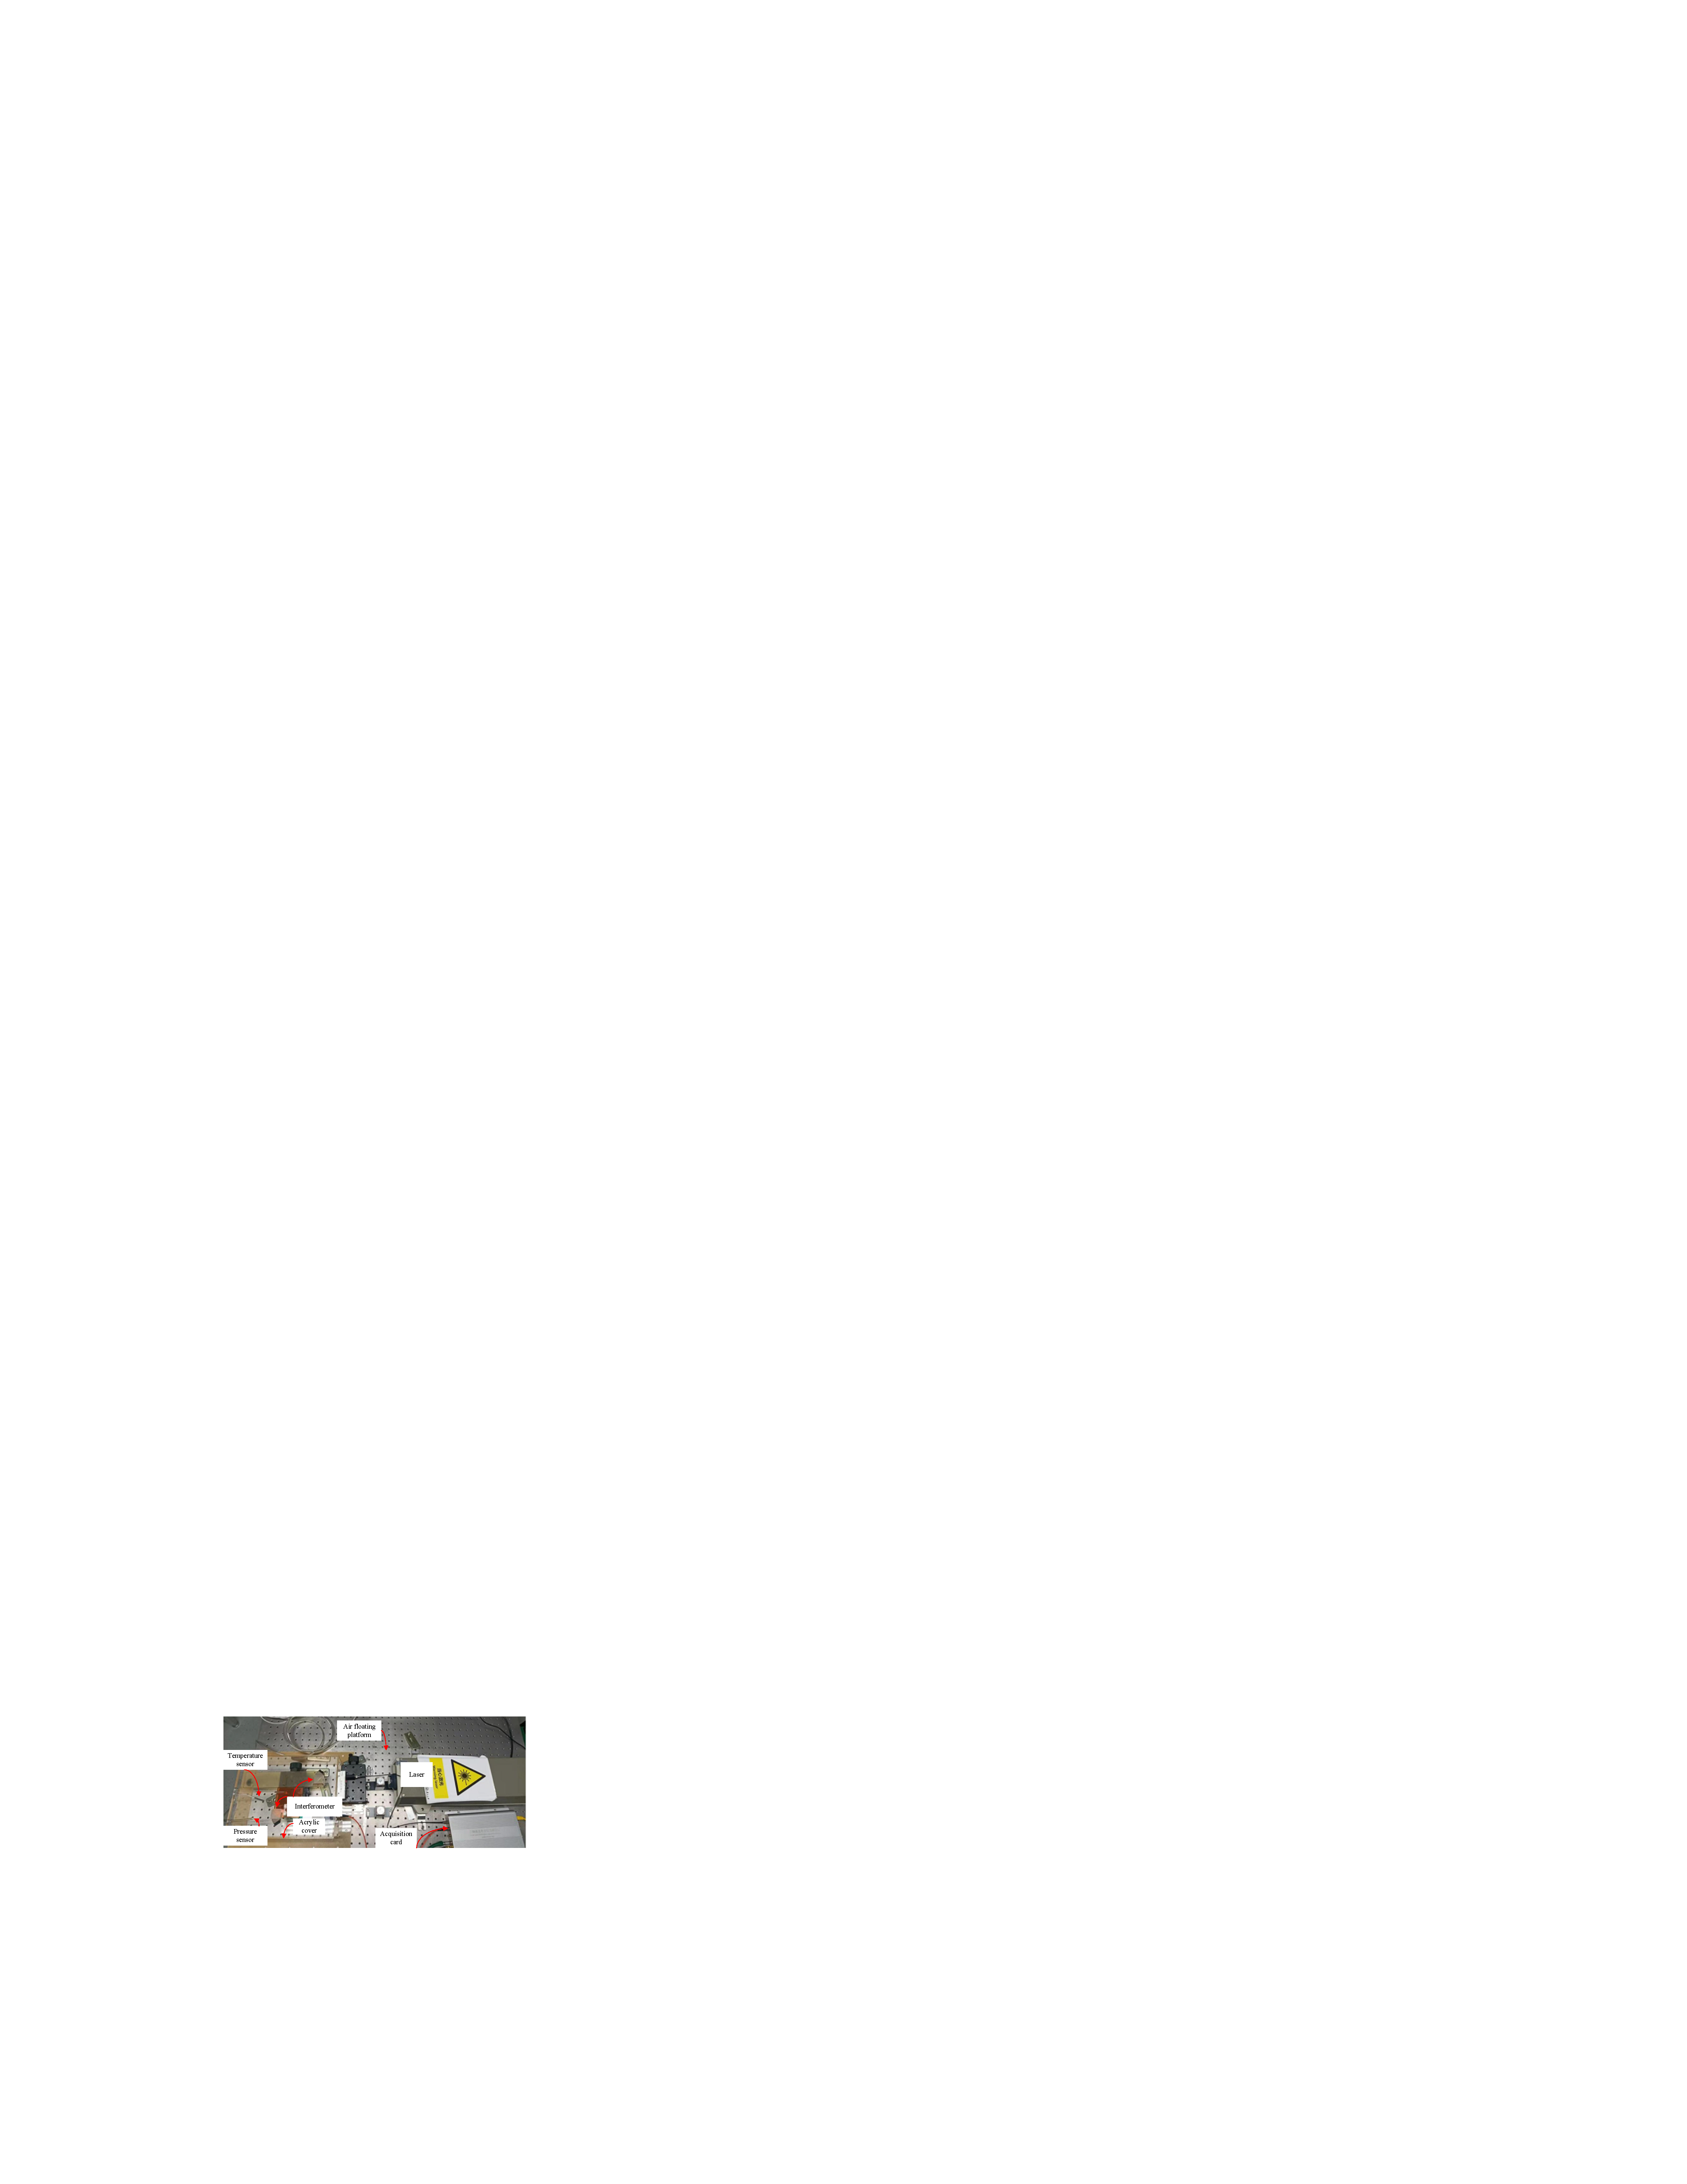
\includegraphics[width=14cm,height=7cm]{fig/3-fig/最终实验系统图.pdf}
      \end{minipage}
      \label{fig:最终实验系统图}
    }
    \caption{最终实验方案}
    \label{fig:最终实验方案}
  \end{figure}

\section{实验系统安装和调试}
上述实验系统的搭建时,主要按照以下基本流程进行:
\begin{enumerate}
    \item 将激光器放置在光学平台上,并进行固定,通电点亮激光器进行预热,待激光器尾部的指示灯亮起时说明预热结束,然后再次固定激光器。
    \item 将分光镜、干涉仪放置在光学平台上,并进行预固定。旋转激光器出口光阑,选择大光斑,随后调分光镜的的位置,确保光束从分光镜外壳通光孔的中心入射,并且没有出现消光现象,然后将激光器的光斑从大光斑调整为小光斑,调整干涉仪位置,确保干涉仪的反射镜与入射光束垂直;随后微调分光镜俯仰角以及干涉仪位置,使得干涉仪的测量光斑和参考光斑重合,并且光斑形状为圆形,然后固定分光镜和干涉仪位置。并将激光器的光斑调整为合适测量的光斑大小。
    \item 将亚克力罩罩在干涉仪上方,并且固定温度传感器和压力传感器,随后将亚克力罩也固定在光学平台上。
    \item 安装光纤耦合器,并将光纤接到采集板卡。
  \end{enumerate}
  \section{补偿性能测试与实验结果}
为了验证Edlen公式在波长不匹配、温度范围不匹配的情况下,仍然能对干涉仪的环境误差进行一定程度的补偿,但会使得精度所损失,进行了多次实验数据采集,部分结果如下文所述。所有实验的采样周期均为2s,所有测量均为零位测量,即理论位移应为0。并且从式\eqref{eq:环境误差公式}可以看出,干涉仪的环境误差是与测量臂长度成正比的,而其它误差(例如随机误差、非线性误差等)往往都与测量臂长度无关,由此可以得出判断干涉仪环境误差补偿是否精准的标志就是看补偿后的残差是否一致。

\subsection{短时测量}
如图\ref{fig:短时测量实验数据}所示,(a)图为测量臂长度为45mm的位移测量数据,(b)图为测量臂长度为90mm的位移测量数据,(c)图为对应的温度和气压数据,(a)、(b)、(c)三图的横轴均为时间,单位为h;(a)和(b)图中的竖轴为位移数据,单位为nm,其中带圆圈标注的蓝色曲线为原始的位移测量数据,带黄色方块标注的为使用原始Edlen公式补偿后的位移数据,(c)图的竖轴为温度和气压数据,单位为$^{\circ} \mathrm{C}$和kPa,其中带圆圈标注的蓝色曲线为温度数据,红色曲线为气压数据。
\begin{figure}[htb]
    \centering
    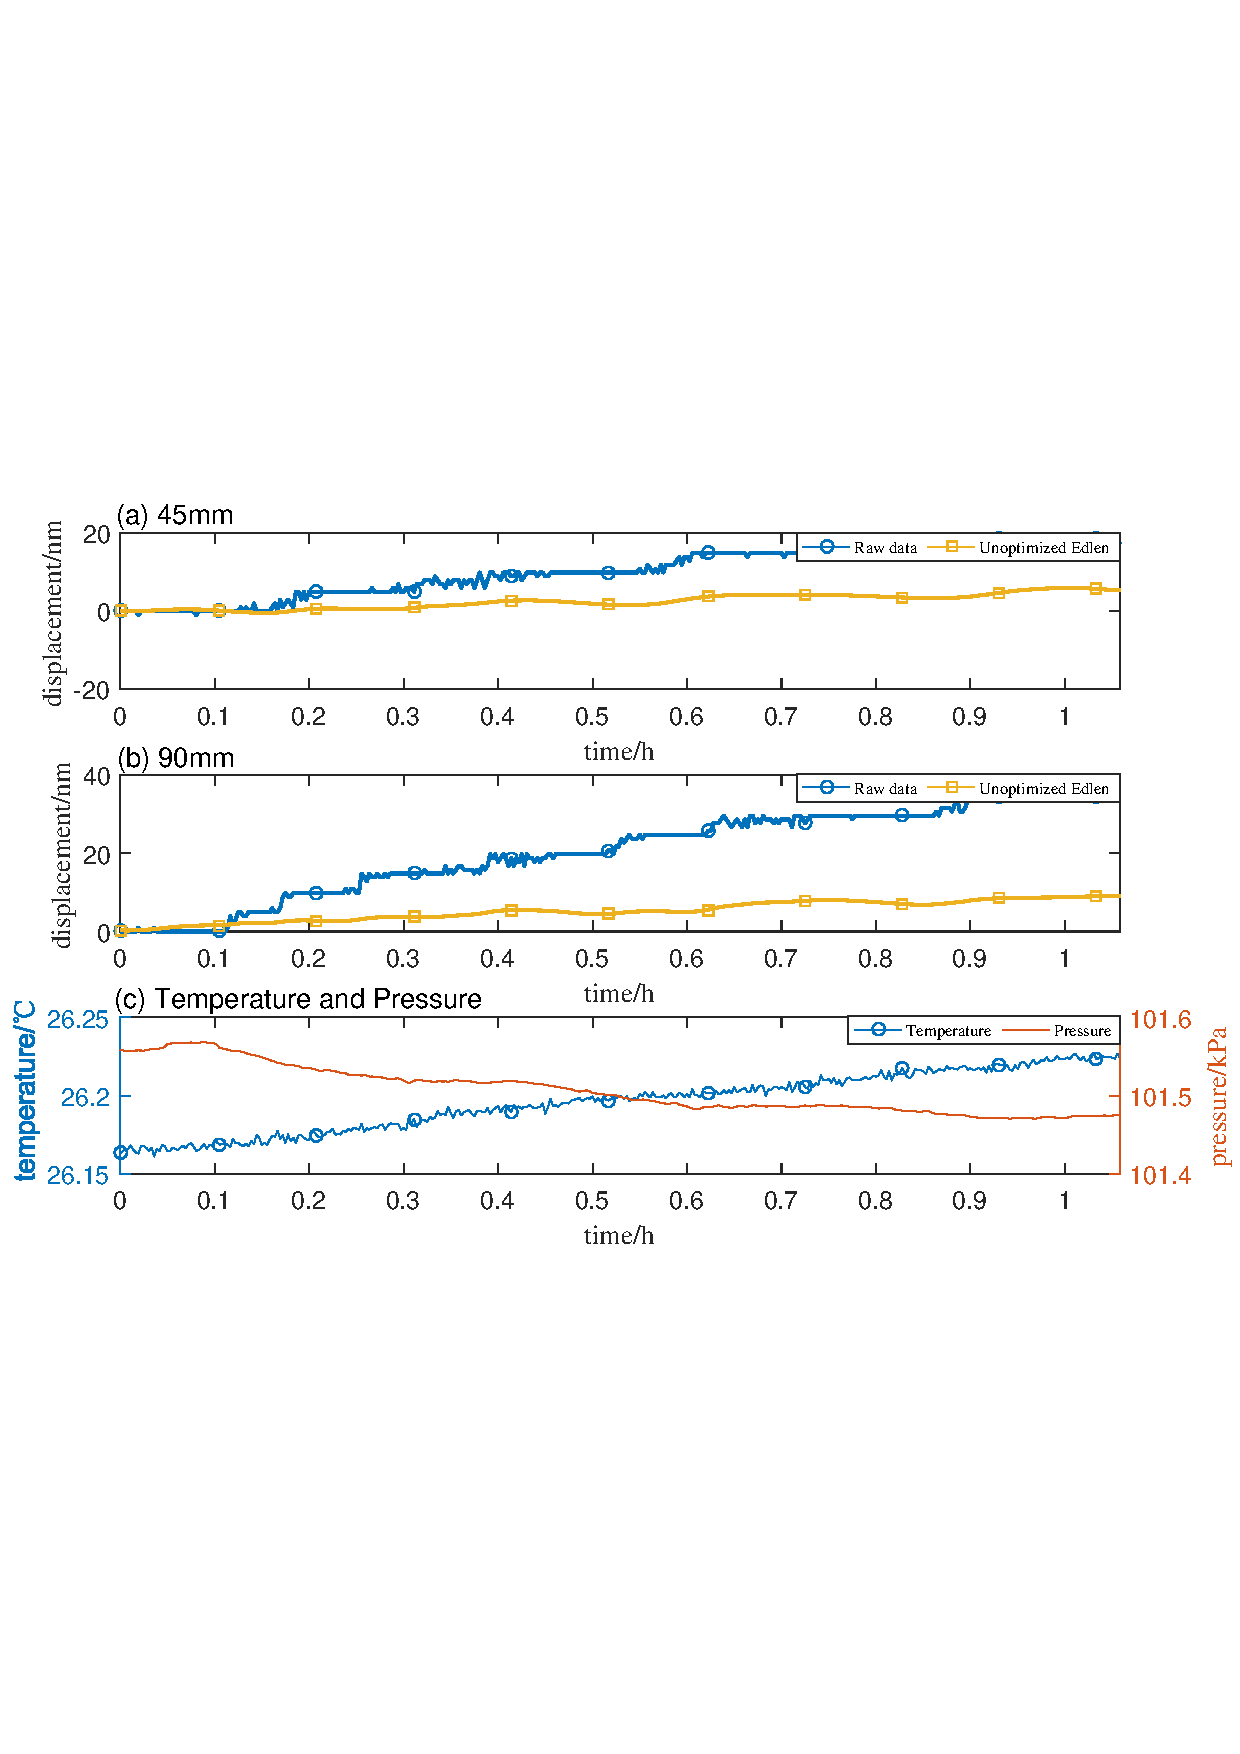
\includegraphics[width=14cm]{fig/3-fig/短时测量数据.pdf}
    \caption{短时测量实验数据}
    \label{fig:短时测量实验数据}
\end{figure}
从图中可以看出,测量时间约为1h,温度变化范围为$[26.16\,\,\,26.23]^{\circ} \mathrm{C}$,气压变化范围为$[101.6\,\,\,101.5]$kPa,测量臂长度为45mm和90mm的两套干涉仪的原始位移数据的变化范围为$[0\,\,\,19.78]$nm和$[0\,\,\,34.62]$nm,在考虑可能含有随机误差等其他误差的情况下,可近似认为两者成两倍关系。并且对于零位测量而言,上述位移变化都可以认为是误差,对应的均方根误差分别为$11.8869$nm和$23.3770$nm,也符合式\eqref{eq:环境误差公式}中描述的关系,这也说明在测量过程中并未引入太多其他误差,导致干涉仪测量值变化的主要原因为环境因素。

经过Edlen公式补偿后的均方根误差为3.1377nm和5.8401nm,补偿效果约为$71\%$和$75\%$。可以看出使用Edlen公式进行干涉仪的环境误差补偿可以得到较好的补偿效果,但是经过Edlen公式补偿之后的残留均方根误差仍然近似成两倍关系,这说明由于温度不匹配、波长不匹配以及Edlen公式人为总结的局限性,使得Edlen公式在补偿后仍有部分环境误差残留。

\subsection{长时测量}
短时测量的时间1h左右,为了探究Edlen公式在长时间测量情况下的补偿效果,将测量时间增加到7.5h,得到的实验数据如图\ref{fig:长时测量实验数据}。
\begin{figure}[htb]
  \centering
  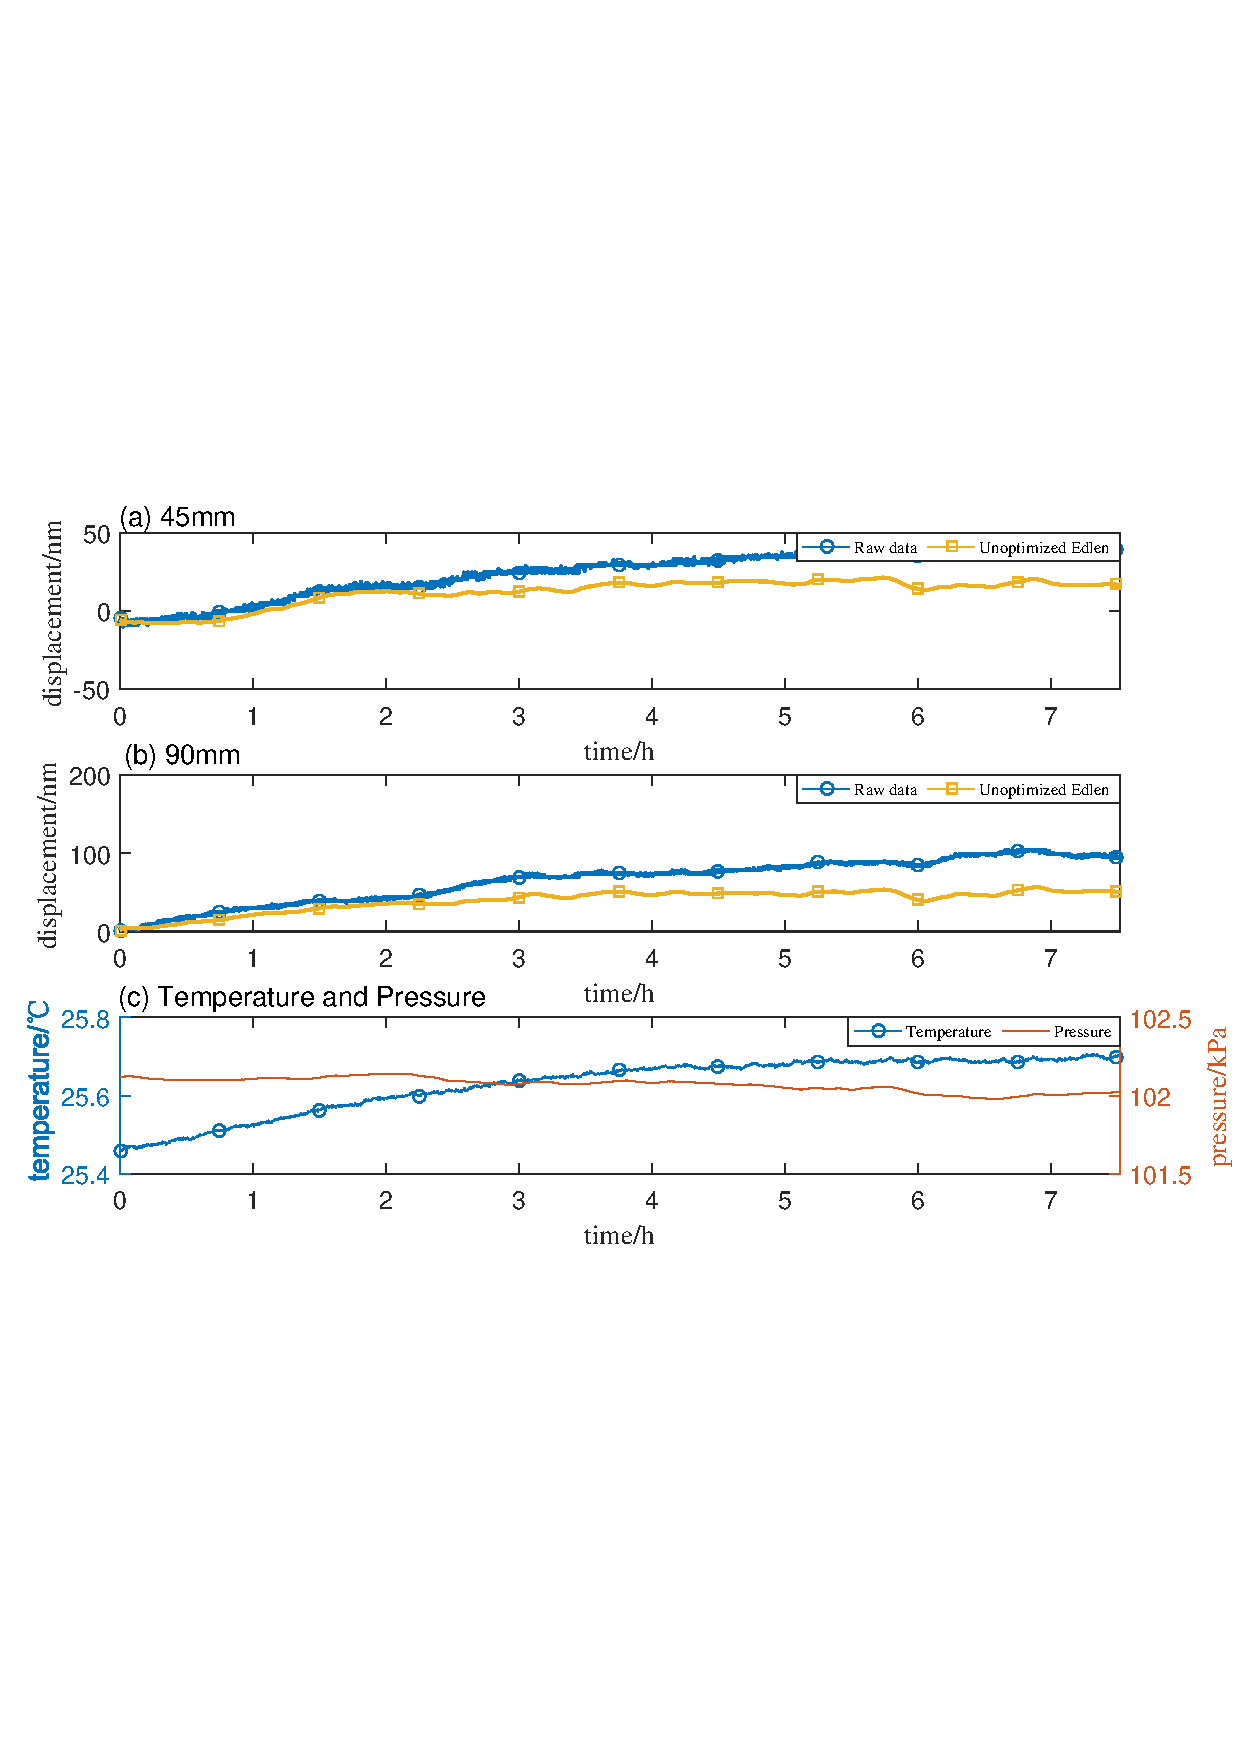
\includegraphics[width=14cm]{fig/3-fig/长时测量数据.pdf}
  \caption{长时测量实验数据}
  \label{fig:长时测量实验数据}
\end{figure}

从图中可以看出,测量时间约为7.5h,温度变化范围为$[25.46\,\,\,25.69]^{\circ} \mathrm{C}$,气压变化范围为$[102.0\,\,\,102.1]$kPa,测量臂长度为45mm和90mm的两套干涉仪的原始位移数据的变化范围为$[0\,\,\,35.62]$nm和$[0\,\,\,89.01]$nm,在考虑可能含有随机误差等其他误差的情况下,可近似认为两者成两倍关系。并且对于零位测量而言,上述位移变化都可以认为是误差,对应的均方根误差分别为30.5299nm和75.0362nm,经过Edlen公式补偿后的均方根误差为14.9957nm和41.9108nm,补偿效果约为$50.8\%$和$45\%$。

可以看出在进行长时间测量的情况下使用Edlen公式进行干涉仪的环境误差补偿也可以取得一定的补偿效果,但是补偿效果并没有短时测量的效果好,应是测量时间增长使得温度、气压、位移的累计测量误差变大导致,除此之外,仍可以发现补偿后的残留均方根误差依旧有一定差距,补偿效果有提升空间。

\subsection{大范围温度变化测量}
为了更加验证原始Edlen公式由于其温度不匹配问题造成的使用局限性,将测量时温度温度设置的更加远离Edlen公式的提出温度$20^{\circ} \mathrm{C}$,并且增大温度变化区间,进一步增加测量时间,得到的实验数据如图\ref{fig:大范围温度测量实验数据}。
\begin{figure}[htb]
    \centering
    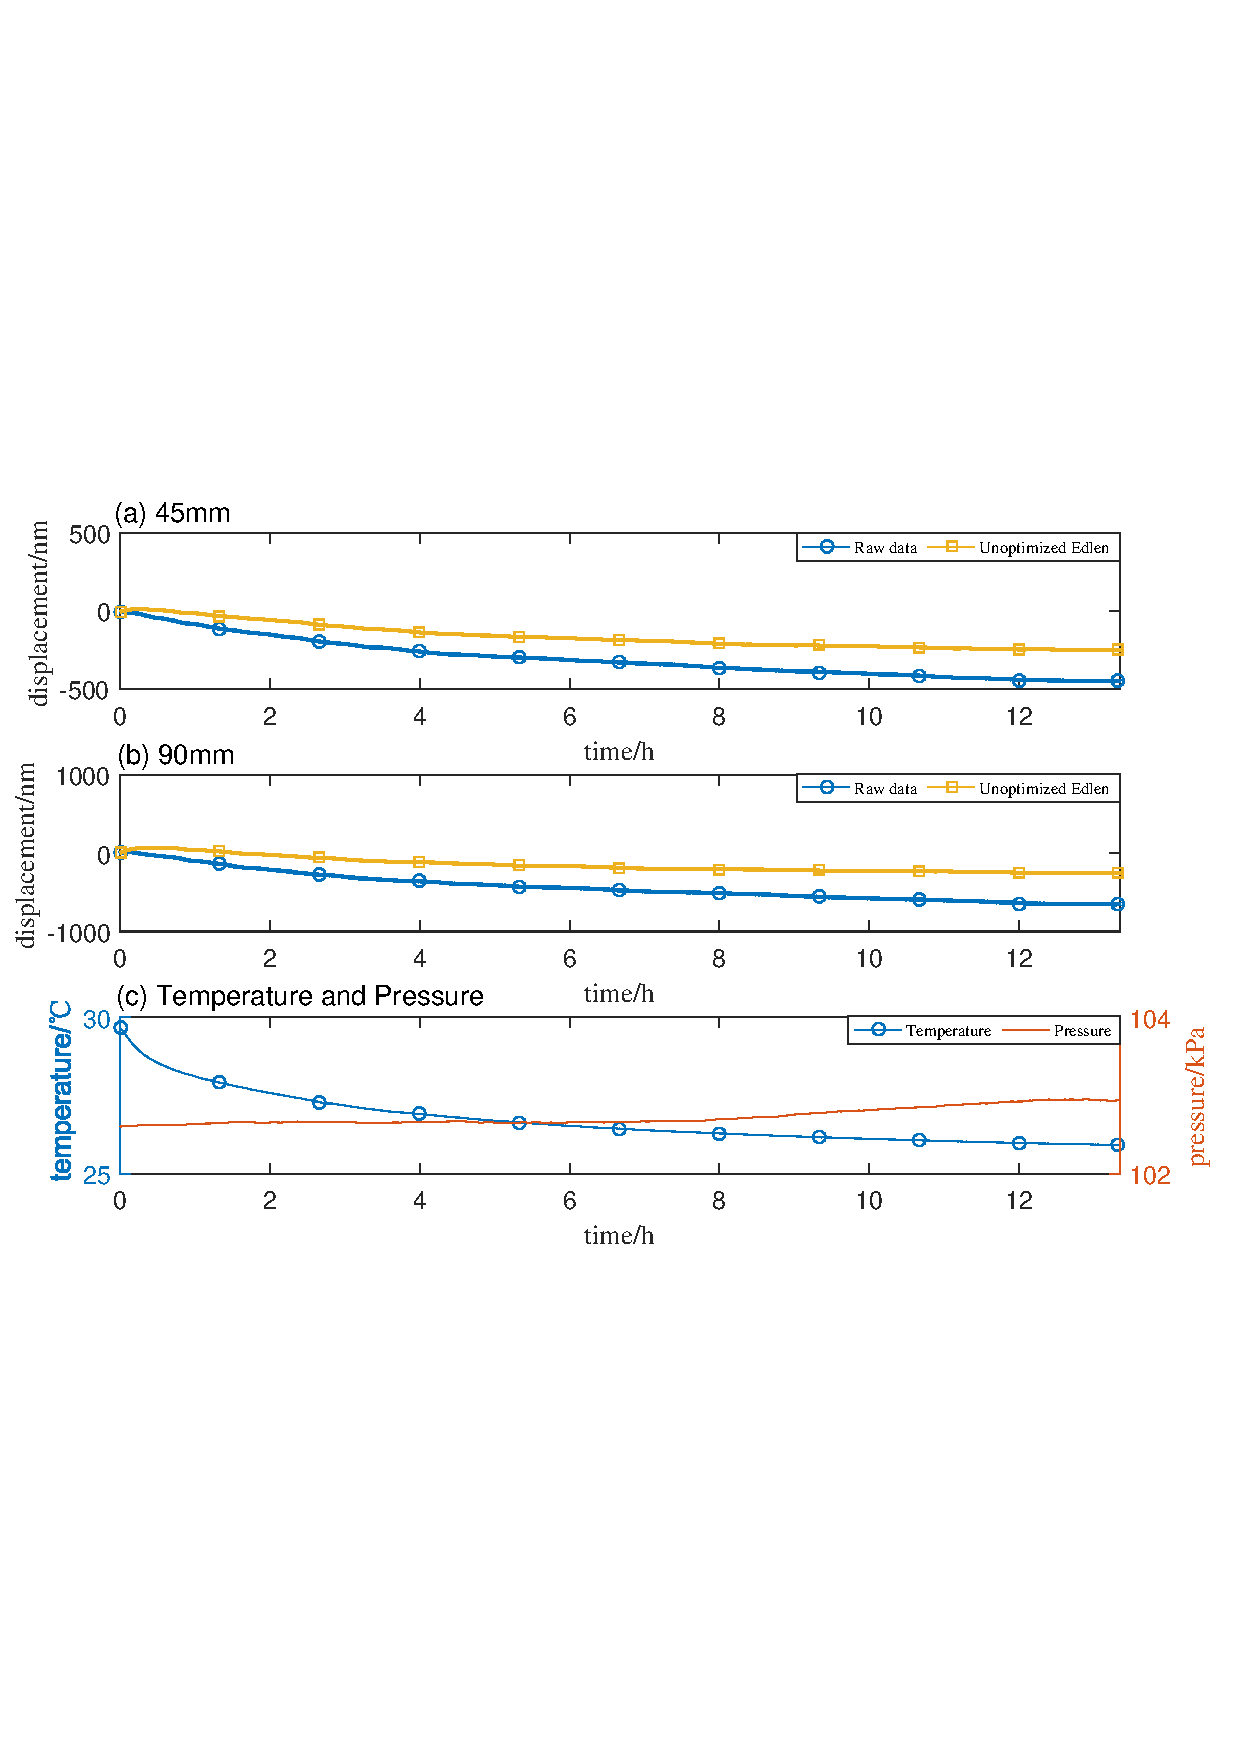
\includegraphics[width=14cm]{fig/3-fig/大范围温度测量实验数据.pdf}
    \caption{大范围温度测量实验数据}
    \label{fig:大范围温度测量实验数据}
  \end{figure}
从图中可以看出,测量时间约为12.5h,温度变化范围为$[25.91\,\,\,29.67]^{\circ} \mathrm{C}$,气压变化范围为$[102.6\,\,\,102.9]$kPa,测量臂长度为45mm和90mm的两套干涉仪的原始位移数据的变化范围为$[0 \,\,\, -248.3]$nm和$[0\,\,\,-652.8]$nm,在考虑可能含有随机误差等其他误差的情况下,可近似认为两者成两倍关系。并且对于零位测量而言,上述位移变化都可以认为是误差,对应的均方根误差分别为325.0990nm和465.0772nm。经过Edlen公式补偿后的均方根误差为153.6245nm和176.6071nm,补偿效果约为$53\%$和$62\%$。

可以看出使用Edlen公式进行干涉仪的环境误差补偿可以得到较好的补偿效果,但是经过Edlen公式补偿之后的残留均方根误差仍有较大差距,并且相比于短时测量的差值2.7024nm而言,由于温度更加远离$20^{\circ} \mathrm{C}$,并且温度变化范围也更大了,导致残留误差的差值也增大到了22.983nm,再次验证了温度不匹配导致原始Edlen公式的补偿效果降低。

从图中还可以看出,在前0.8h的测量时间段内,经过Edlen公式补偿后的值有一个正向的凸起,高度约为70nm(测量臂长度90mm的数据),而干涉仪的位移测量值一直都是处于负数范围内,此时补偿结果的变化趋势是与干涉仪位移值的变化趋势相反的,即由于进行了补偿,导致干涉仪的位移值从负数跨越零点达到正数,并且距离零点有一点距离,这说明发生了过补偿的现象。但在剩余12h的测量时间内,补偿结果的变化趋势是与干涉仪位移值的变化趋势都是相同的(即变小)。从(c)图中可以看出,前0.8h时间内,测量温度是最远离Edlen公式的提出温度$20^{\circ} \mathrm{C}$,这段时间内发生过补偿进一步说明了温度不匹配造成Edlen公式补偿效果的下降。而且这0.8h内温度从$29.67^{\circ} \mathrm{C}$减小到了$28.22^{\circ} \mathrm{C}$,即在约$6.4\%$的时间内,完成了约整个过程约$38.6\%$的温度变化,这一数据说明,当温度梯度过大时,可能会对干涉仪的位移测量引入其他误差,这部分将在下文介绍。

\section{本章小结}
本章主要介绍了实验系统的搭建以及实验的进行,包括:
\begin{enumerate}
  \item 双频激光干涉仪的光路设计及其分析。
  \item 基于PT100的多通道温度测量系统,包含其上位机软件以及标定过程和标定结果、PACE1000气压传感器。
  \item 介绍了部分不太完善的实验方案及其结果分析,从实验设备、实验变量、实验环境以及实验方法四个方面不断改进,并得到最终的实验方案。
  \item 进行了短时测量、长时测量等对照实验,从具体的数据分析验证了Edlen公式在波长不匹配、温度范围不匹配的情况下,仍然能对干涉仪的环境误差进行一定程度的补偿,但会有一定的性能损失。
\end{enumerate}
